\documentclass[aspectratio=169,10pt]{beamer}
\makeatletter\def\input@path{{theme/}}\makeatother
\usetheme[nosectionpages]{SwissAstro}
\usepackage[french]{babel}
\setbeamertemplate{frametitle}{\vspace{2.4mm}\noindent\usebeamerfont{frametitle}\insertframetitle\par\vspace{1mm}\color{SwissInk}\rule{\linewidth}{.6pt}\par}
\title[Vibe coding en astronomie]{Le vibe coding pour l'astronomie amateur}
\author{Steve Prud'Homme}
\date{Conférence-atelier}
\begin{document}
\begin{frame}{Le vibe coding pour l'astronomie amateur}
\vspace{-0.6mm}{\scriptsize\color{SwissMuted}0:00 – 0:02 · 2 min}\par\smallskip
\begin{columns}[T,onlytextwidth]\begin{column}{.38\textwidth}\raggedright\fontsize{9.6}{12}\selectfont
{\color{SwissAccent}\rule{6mm}{1pt}}\par\medskip
Créer ses propres logiciels libres à partir d'un besoin d'observation.\par\medskip
Steve Prud'Homme · Conférence-atelier · 2 heures\par\medskip
\end{column}\begin{column}{.60\textwidth}\centering
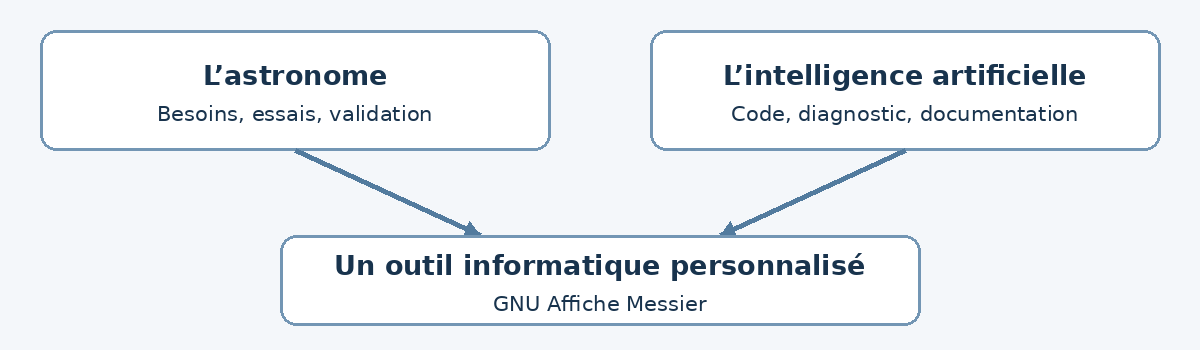
\includegraphics[width=1\linewidth,height=48mm,keepaspectratio]{figures/image1.png}%
\end{column}\end{columns}
\end{frame}
\begin{frame}{Notre parcours, de l'idée au ciel}
\vspace{-0.6mm}{\scriptsize\color{SwissMuted}0:02 – 0:05 · 3 min}\par\smallskip
\begin{columns}[T,onlytextwidth]\begin{column}{.38\textwidth}\raggedright\fontsize{9.6}{12}\selectfont
{\color{SwissAccent}\rule{6mm}{1pt}}\par\medskip
Choisir une tâche et anticiper les erreurs de l'IA.\par\medskip
Écrire une consigne, tester le logiciel et partager sa première version.\par\medskip
Découvrir quatre projets réalisés avec un Seestar S50.\par\medskip
\end{column}\begin{column}{.60\textwidth}\centering
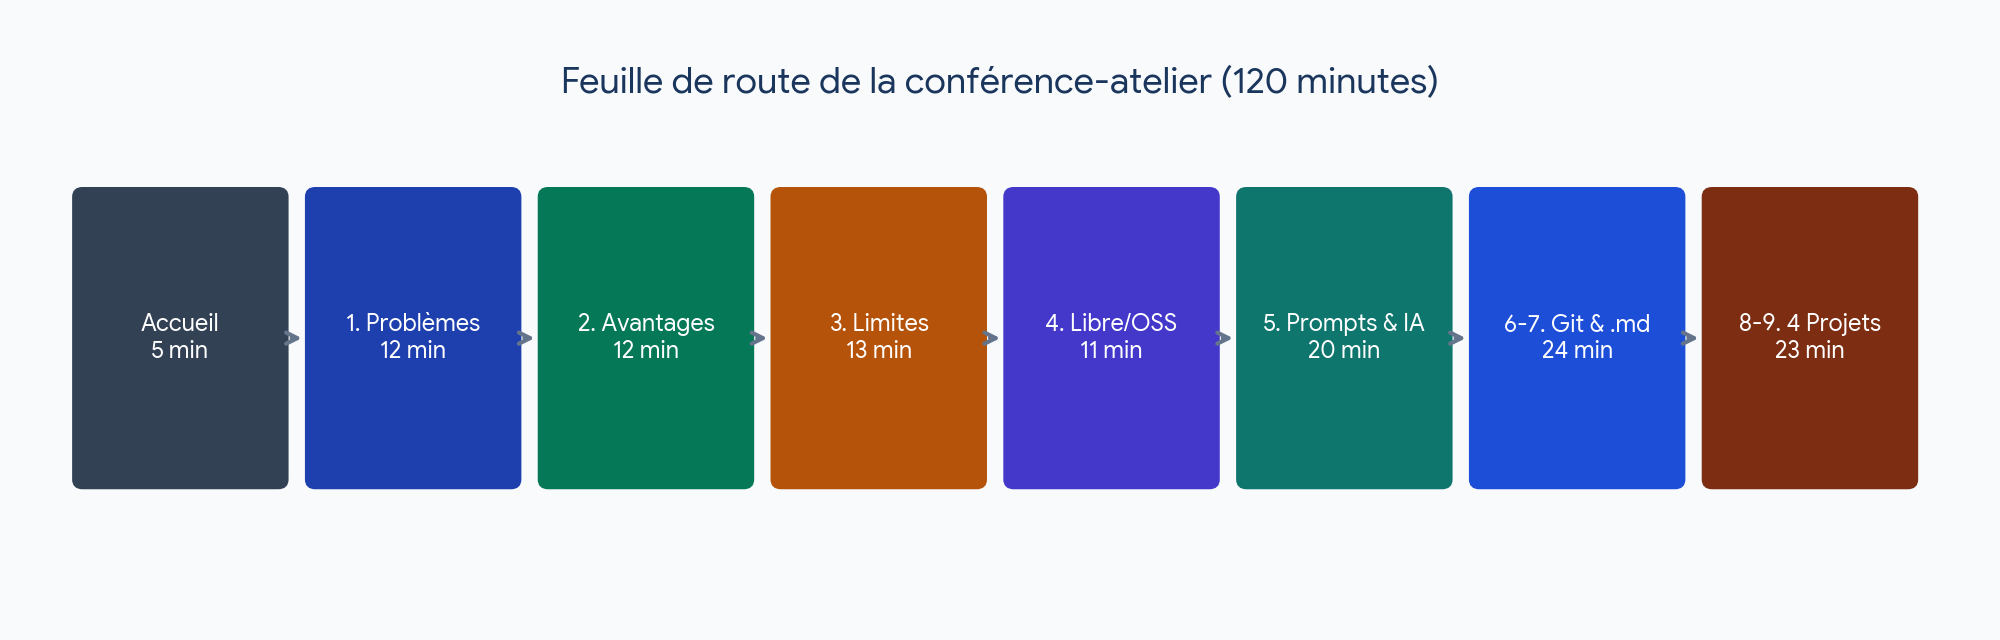
\includegraphics[width=1\linewidth,height=48mm,keepaspectratio]{figures/image2.png}%
\end{column}\end{columns}
\end{frame}
\begin{frame}{Décrire le résultat que l'on cherche}
\vspace{-0.6mm}{\scriptsize\color{SwissMuted}0:05 – 0:08 · 3 min}\par\smallskip
\begin{columns}[T,onlytextwidth]\begin{column}{.38\textwidth}\raggedright\fontsize{9.6}{12}\selectfont
{\color{SwissAccent}\rule{6mm}{1pt}}\par\medskip
« Prépare une liste des cibles visibles depuis mon balcon. »\par\medskip
Indiquez à l'IA ce que vous voulez obtenir. Essayez sa première proposition sur une cible connue.\par\medskip
\end{column}\begin{column}{.60\textwidth}\centering
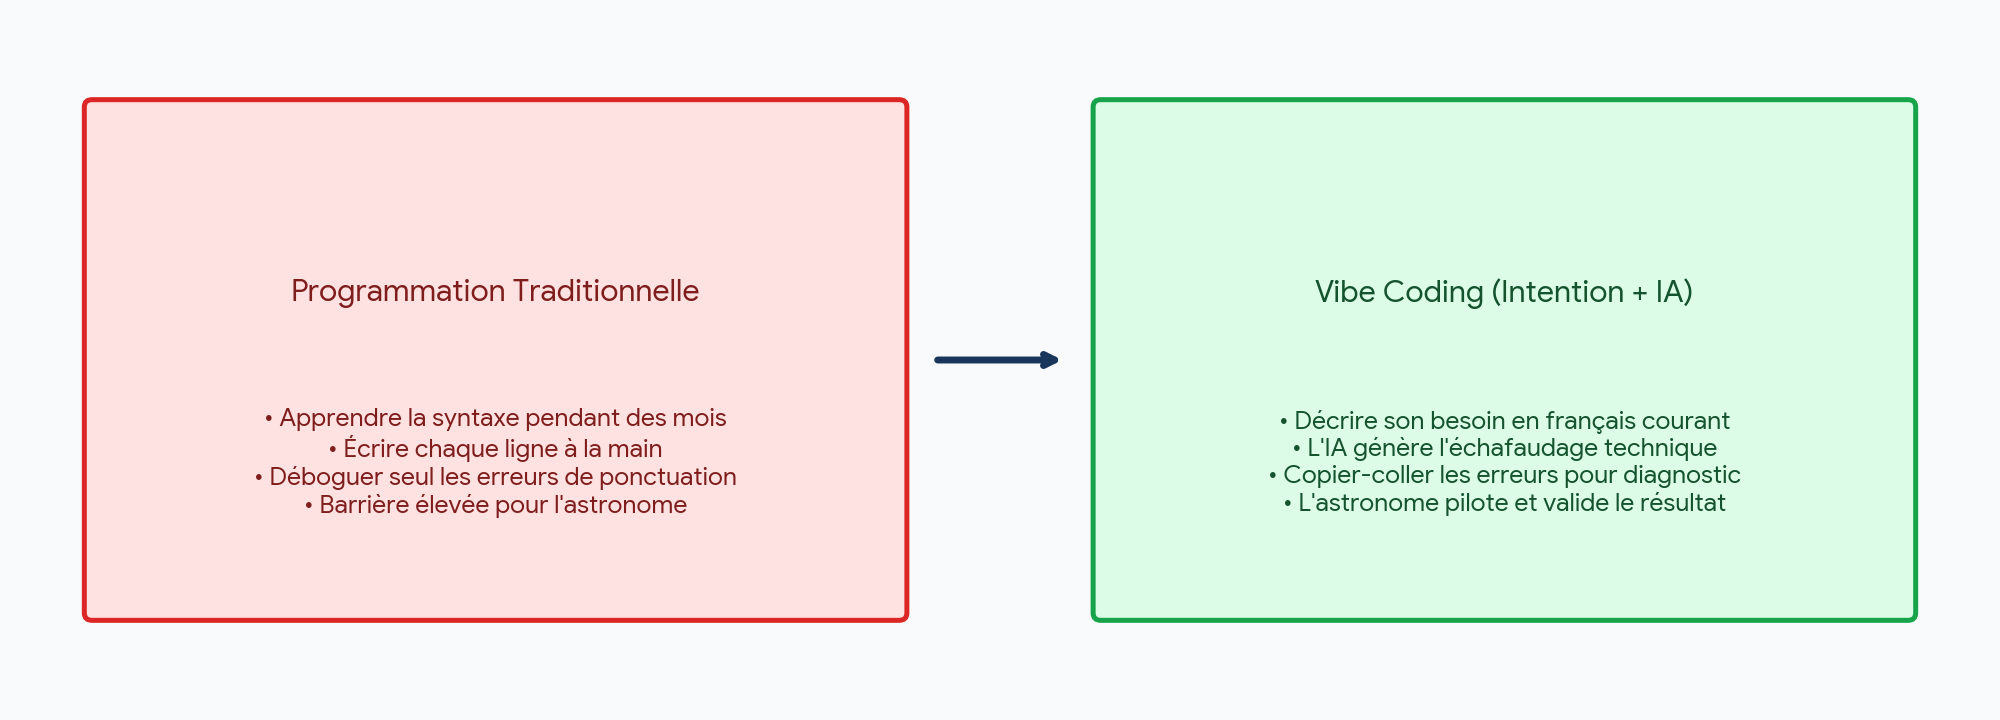
\includegraphics[width=1\linewidth,height=48mm,keepaspectratio]{figures/image3.png}%
\end{column}\end{columns}
\end{frame}
\begin{frame}{Relier des outils déjà éprouvés}
\vspace{-0.6mm}{\scriptsize\color{SwissMuted}0:08 – 0:11 · 3 min}\par\smallskip
\begin{columns}[T,onlytextwidth]\begin{column}{.38\textwidth}\raggedright\fontsize{9.6}{12}\selectfont
{\color{SwissAccent}\rule{6mm}{1pt}}\par\medskip
Un fichier FITS contient une image et les renseignements de la prise de vue.\par\medskip
Astropy lit le fichier. SIMBAD renseigne l'objet. Matplotlib trace la carte.\par\medskip
\end{column}\begin{column}{.60\textwidth}\centering
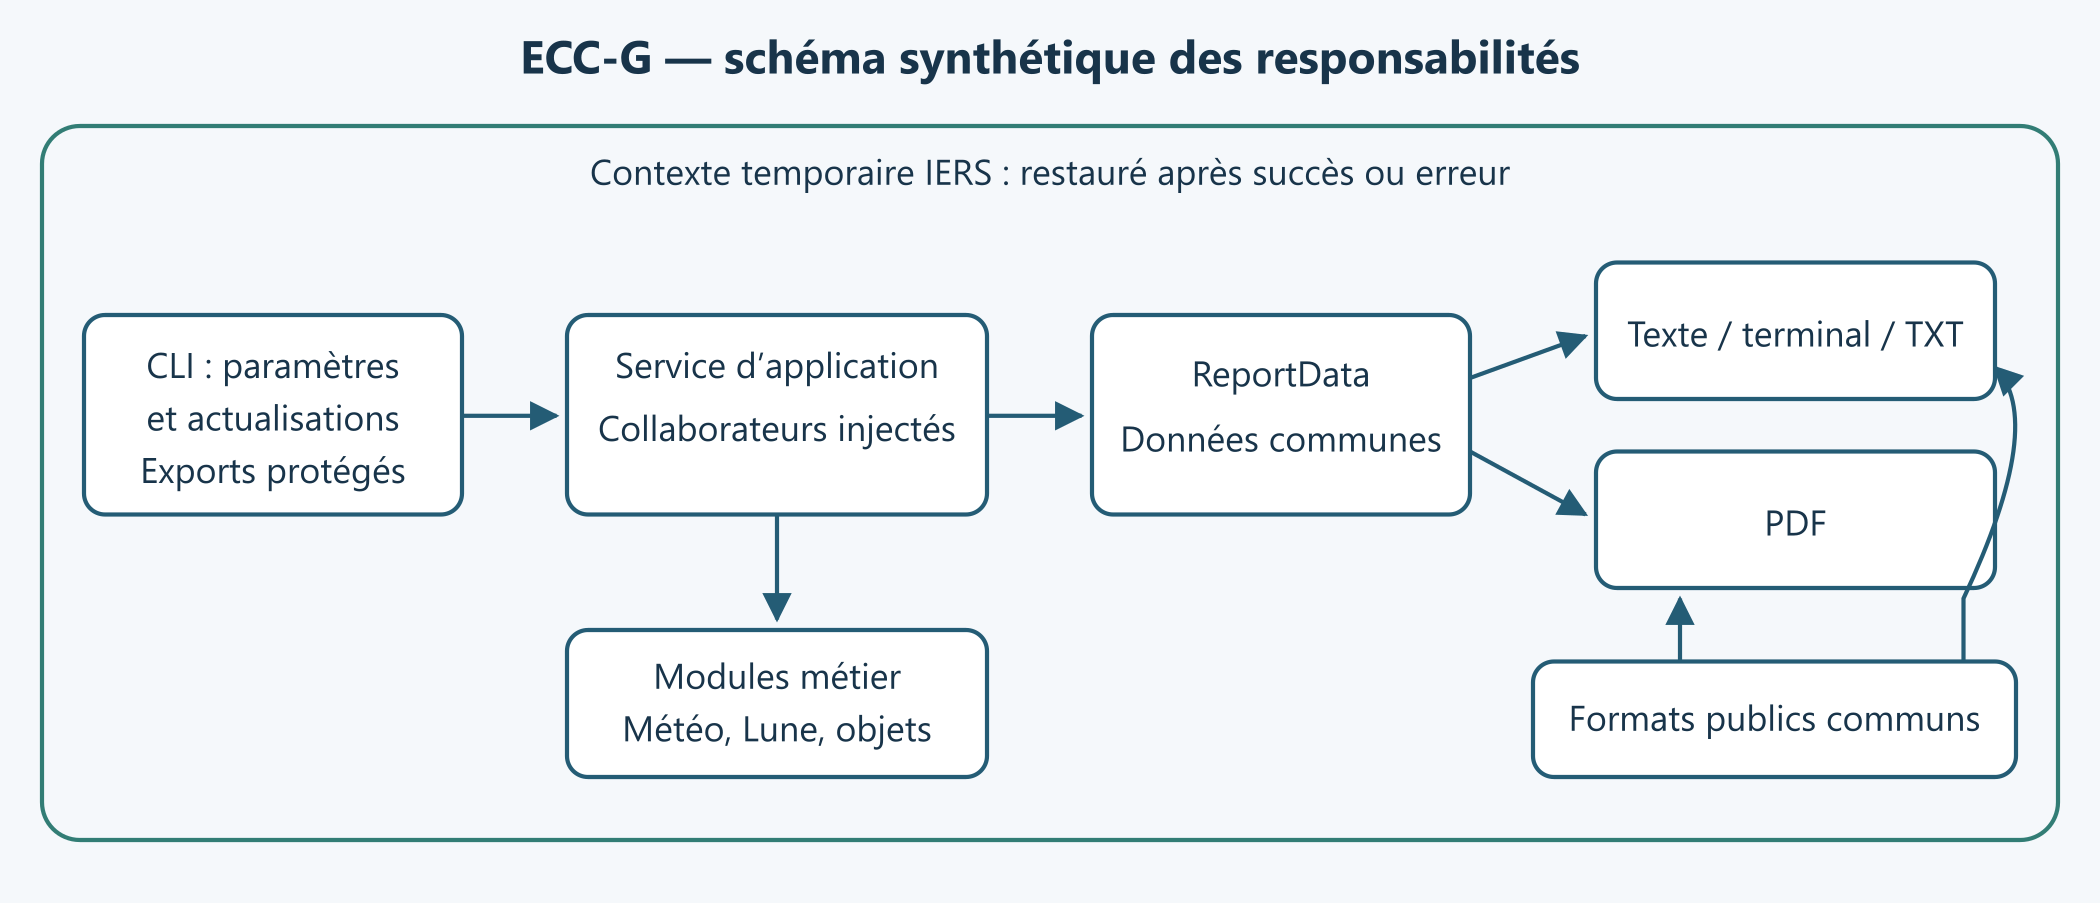
\includegraphics[width=1\linewidth,height=48mm,keepaspectratio]{figures/image4.png}%
\end{column}\end{columns}
\end{frame}
\begin{frame}{Transformer une erreur en indice}
\vspace{-0.6mm}{\scriptsize\color{SwissMuted}0:11 – 0:14 · 3 min}\par\smallskip
\begin{columns}[T,onlytextwidth]\begin{column}{.38\textwidth}\raggedright\fontsize{9.6}{12}\selectfont
{\color{SwissAccent}\rule{6mm}{1pt}}\par\medskip
Copiez le message exact. Précisez la commande et le résultat attendu.\par\medskip
Rejouez le même essai après la correction.\par\medskip
\end{column}\begin{column}{.60\textwidth}\centering
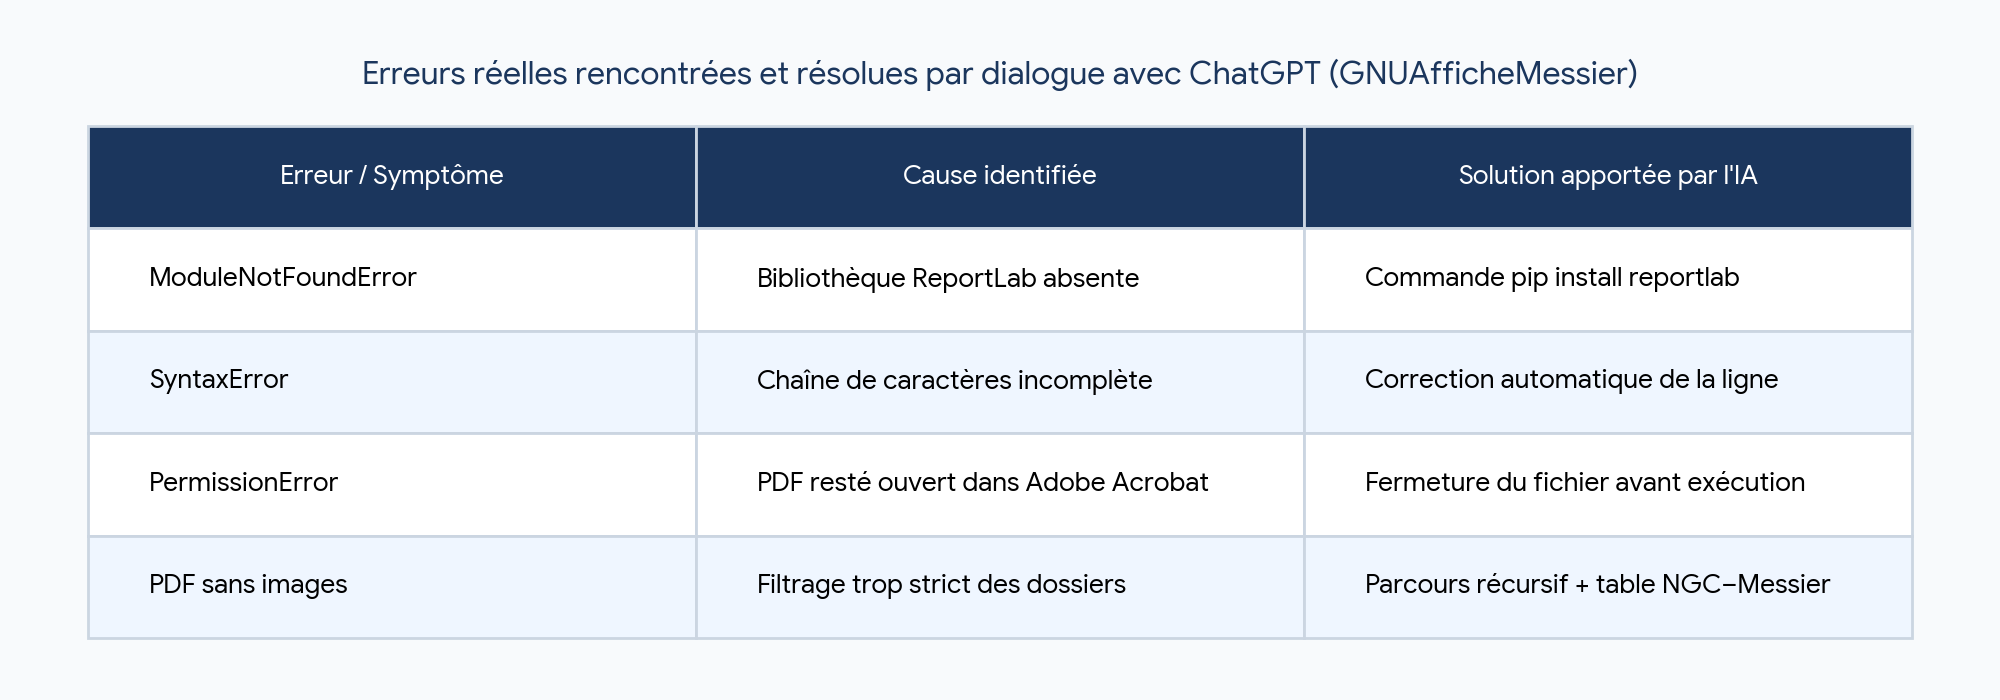
\includegraphics[width=1\linewidth,height=48mm,keepaspectratio]{figures/image5.png}%
\end{column}\end{columns}
\end{frame}
\begin{frame}{Automatiser une tâche répétitive}
\vspace{-0.6mm}{\scriptsize\color{SwissMuted}0:14 – 0:17 · 3 min}\par\smallskip
\begin{columns}[T,onlytextwidth]\begin{column}{.38\textwidth}\raggedright\fontsize{9.6}{12}\selectfont
{\color{SwissAccent}\rule{6mm}{1pt}}\par\medskip
147 images à documenter \(\times\) 10 minutes par image.\par\medskip
24 h 30 de travail manuel estimé. Chronométrez ensuite votre propre série.\par\medskip
\end{column}\begin{column}{.60\textwidth}\centering
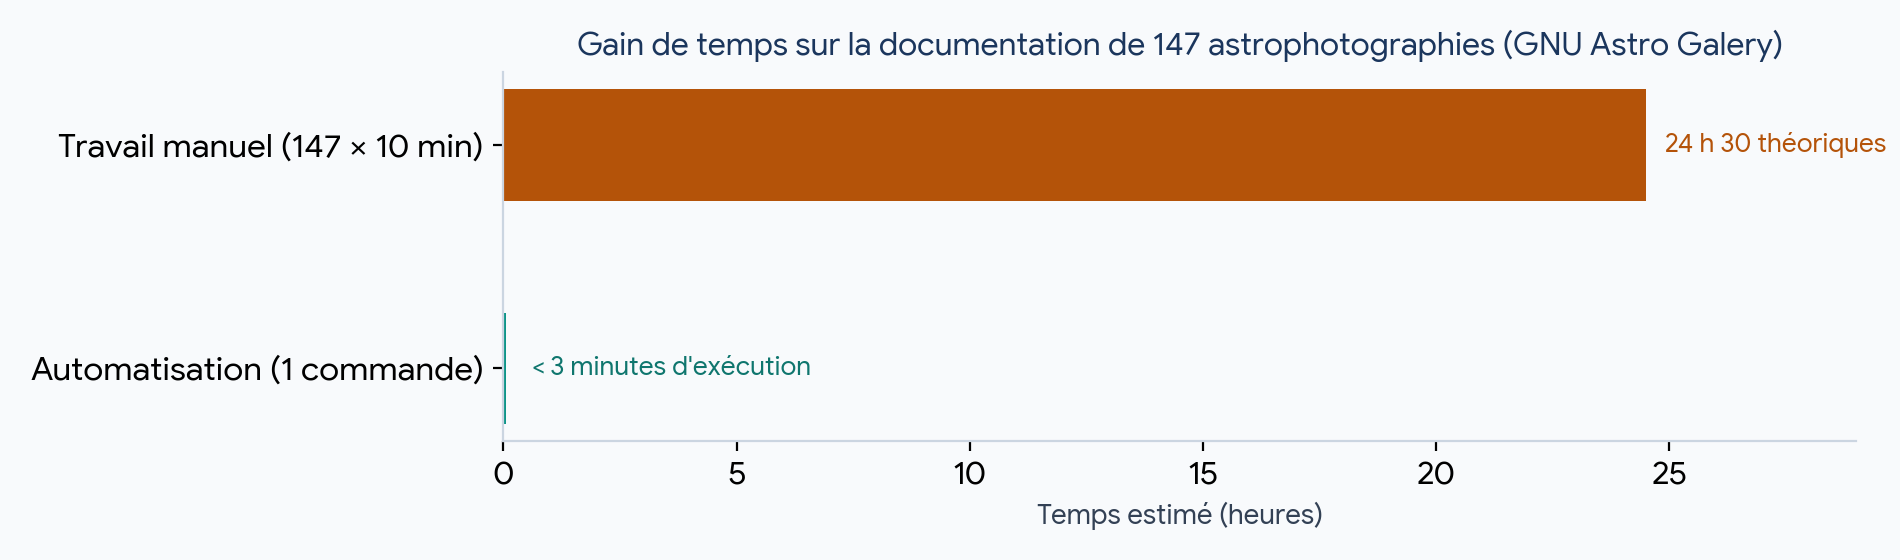
\includegraphics[width=1\linewidth,height=48mm,keepaspectratio]{figures/image6.png}%
\end{column}\end{columns}
\end{frame}
\begin{frame}{Cinq raisons d'essayer le vibe coding}
\vspace{-0.6mm}{\scriptsize\color{SwissMuted}0:17 – 0:19 · 2 min}\par\smallskip
\begin{columns}[T,onlytextwidth]\begin{column}{.38\textwidth}\raggedright\fontsize{9.6}{12}\selectfont
{\color{SwissAccent}\rule{6mm}{1pt}}\par\medskip
FAAFO résume cinq possibilités selon Kim et Yegge.\par\medskip
Rapidité, ambition, autonomie, plaisir et liberté d'essayer plusieurs solutions.\par\medskip
\end{column}\begin{column}{.60\textwidth}\centering
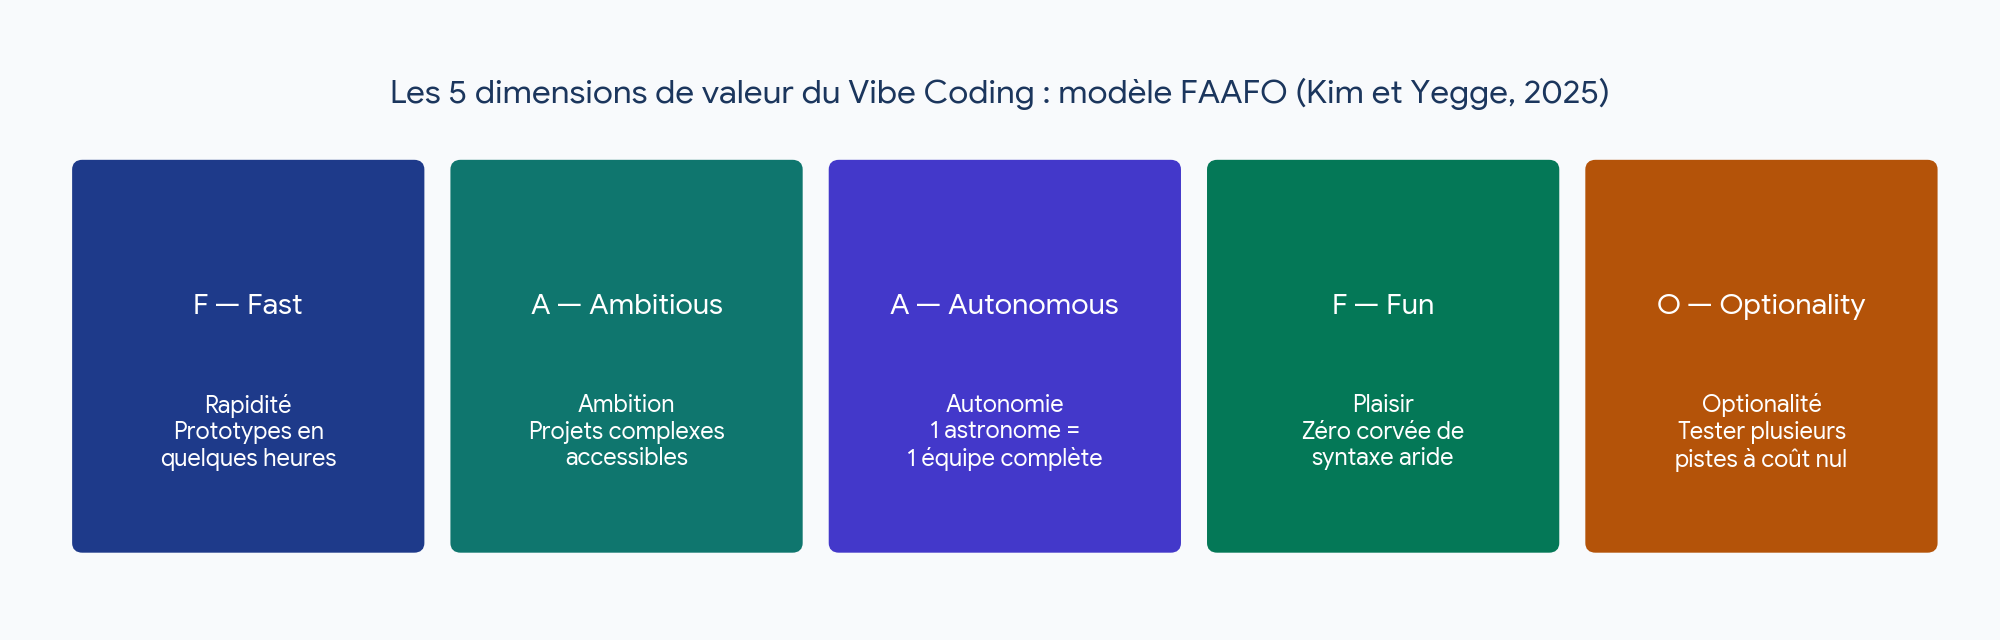
\includegraphics[width=1\linewidth,height=48mm,keepaspectratio]{figures/image7.png}%
\end{column}\end{columns}
\end{frame}
\begin{frame}{Passer d'un catalogue à plusieurs}
\vspace{-0.6mm}{\scriptsize\color{SwissMuted}0:19 – 0:22 · 3 min}\par\smallskip
\begin{columns}[T,onlytextwidth]\begin{column}{.38\textwidth}\raggedright\fontsize{9.6}{12}\selectfont
{\color{SwissAccent}\rule{6mm}{1pt}}\par\medskip
Commencez avec une liste Messier.\par\medskip
Ajoutez le catalogue Caldwell. Vérifiez un objet qui figure déjà dans votre liste.\par\medskip
\end{column}\begin{column}{.60\textwidth}\centering
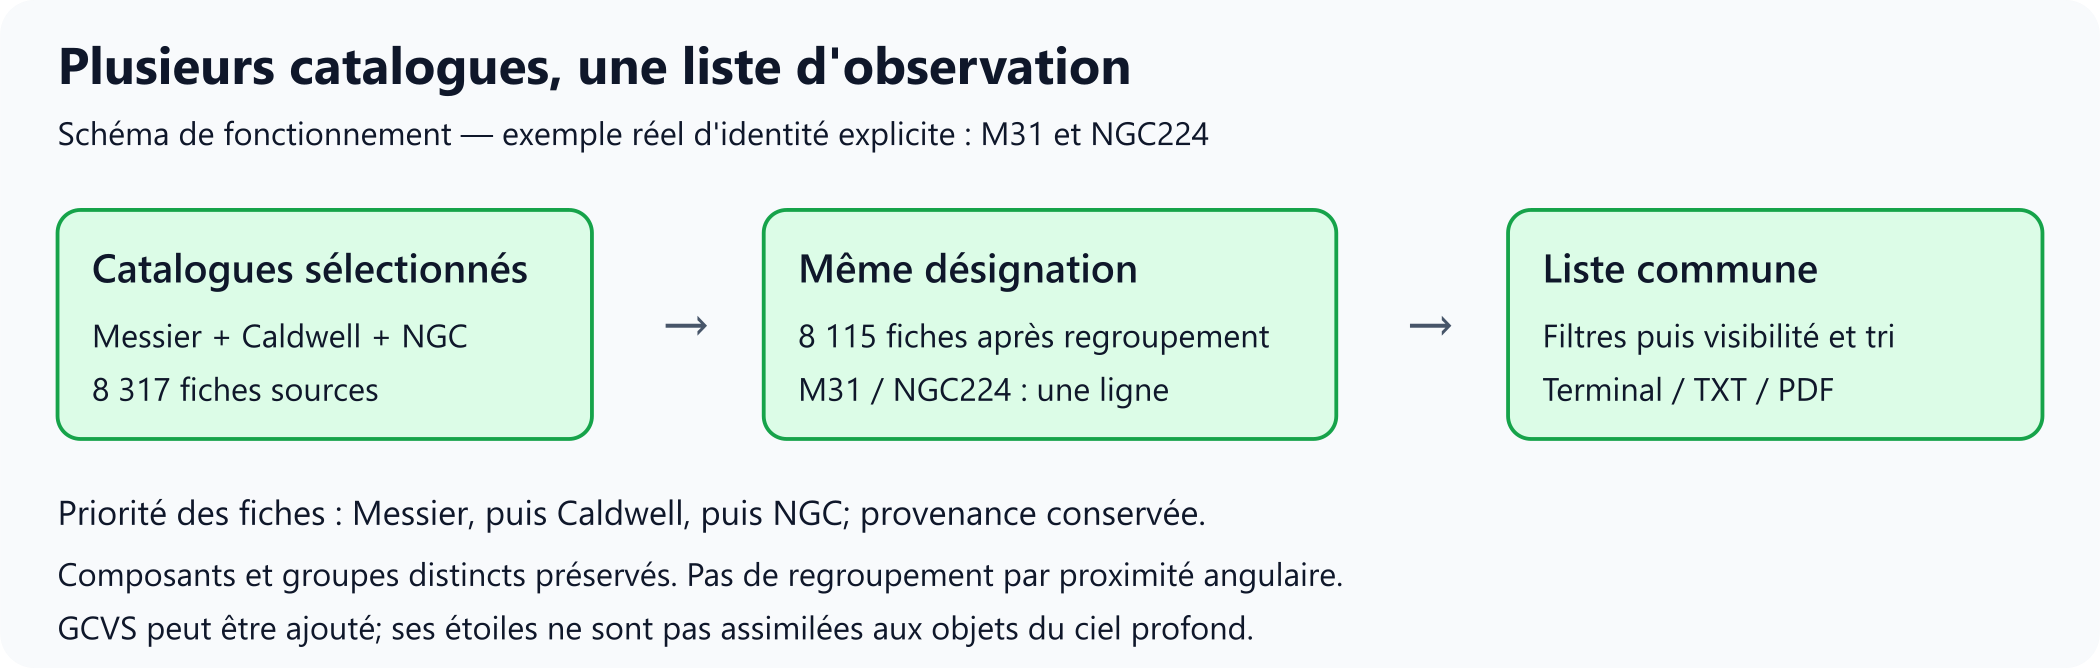
\includegraphics[width=1\linewidth,height=48mm,keepaspectratio]{figures/image8.png}%
\end{column}\end{columns}
\end{frame}
\begin{frame}{Garder la main sur son outil}
\vspace{-0.6mm}{\scriptsize\color{SwissMuted}0:22 – 0:25:30 · 3,5 min}\par\smallskip
\begin{columns}[T,onlytextwidth]\begin{column}{.38\textwidth}\raggedright\fontsize{9.6}{12}\selectfont
{\color{SwissAccent}\rule{6mm}{1pt}}\par\medskip
Un soir nuageux suffit pour essayer une petite idée.\par\medskip
Choisissez une modification que vous pourrez vérifier vous-même.\par\medskip
\end{column}\begin{column}{.60\textwidth}\centering
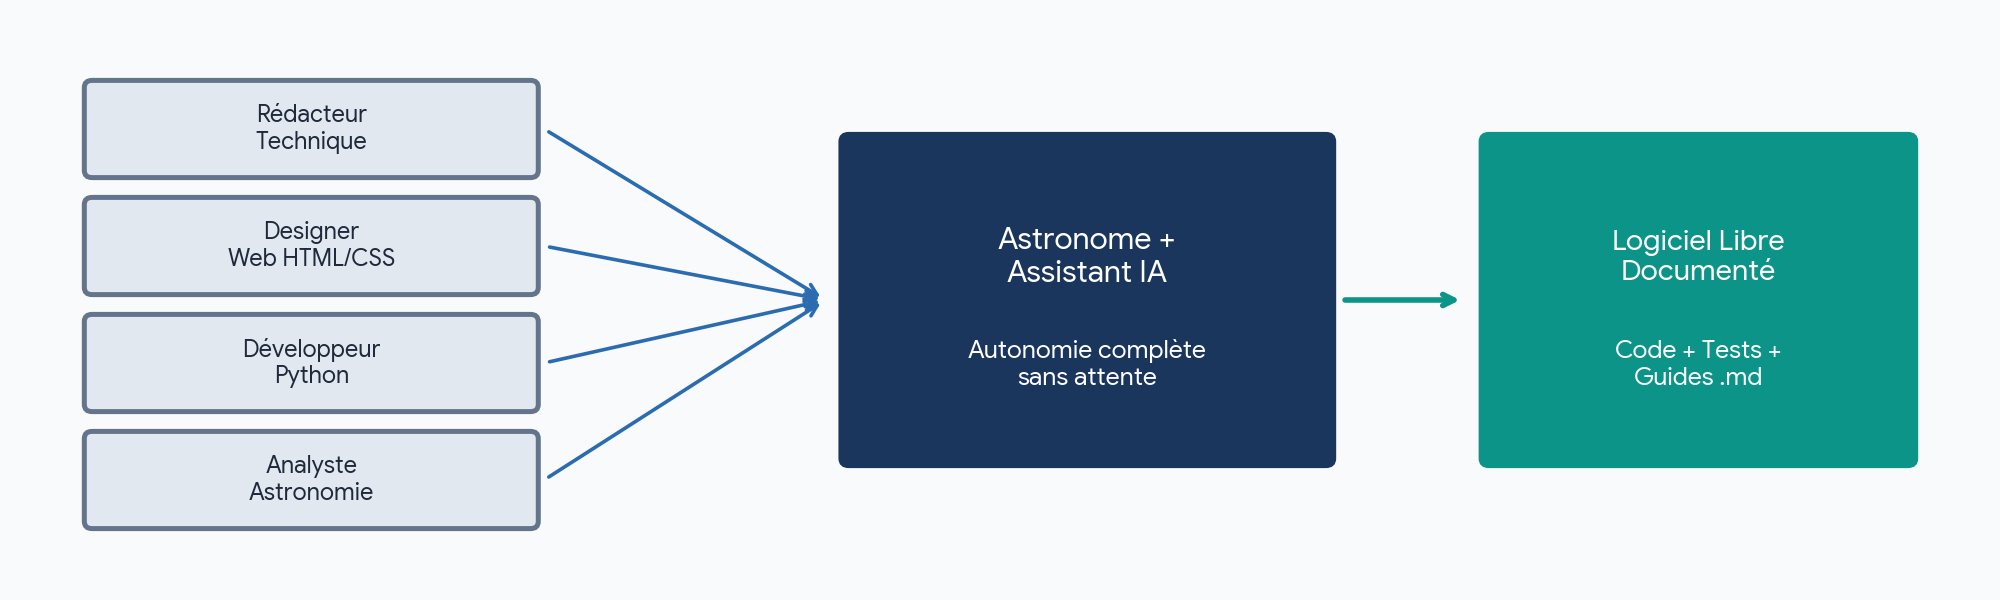
\includegraphics[width=1\linewidth,height=48mm,keepaspectratio]{figures/image9.png}%
\end{column}\end{columns}
\end{frame}
\begin{frame}{Essayer deux solutions au même besoin}
\vspace{-0.6mm}{\scriptsize\color{SwissMuted}0:25:30 – 0:29 · 3,5 min}\par\smallskip
\begin{columns}[T,onlytextwidth]\begin{column}{.38\textwidth}\raggedright\fontsize{9.6}{12}\selectfont
{\color{SwissAccent}\rule{6mm}{1pt}}\par\medskip
Demandez un tableau, puis une carte du même ciel.\par\medskip
Gardez la version qui vous aide à décider quoi observer.\par\medskip
\end{column}\begin{column}{.60\textwidth}\centering
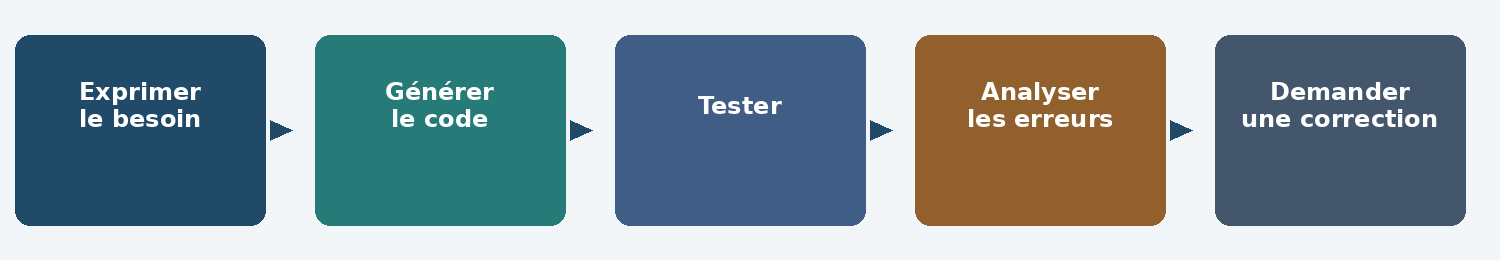
\includegraphics[width=1\linewidth,height=48mm,keepaspectratio]{figures/image10.png}%
\end{column}\end{columns}
\end{frame}
\begin{frame}{Une réponse plausible peut être fausse}
\vspace{-0.6mm}{\scriptsize\color{SwissMuted}0:29 – 0:32:30 · 3,5 min}\par\smallskip
\begin{columns}[T,onlytextwidth]\begin{column}{.38\textwidth}\raggedright\fontsize{9.6}{12}\selectfont
{\color{SwissAccent}\rule{6mm}{1pt}}\par\medskip
Une image bien présentée peut porter le mauvais identifiant.\par\medskip
Comparez le nom et les coordonnées dans un catalogue indépendant.\par\medskip
\end{column}\begin{column}{.60\textwidth}\centering
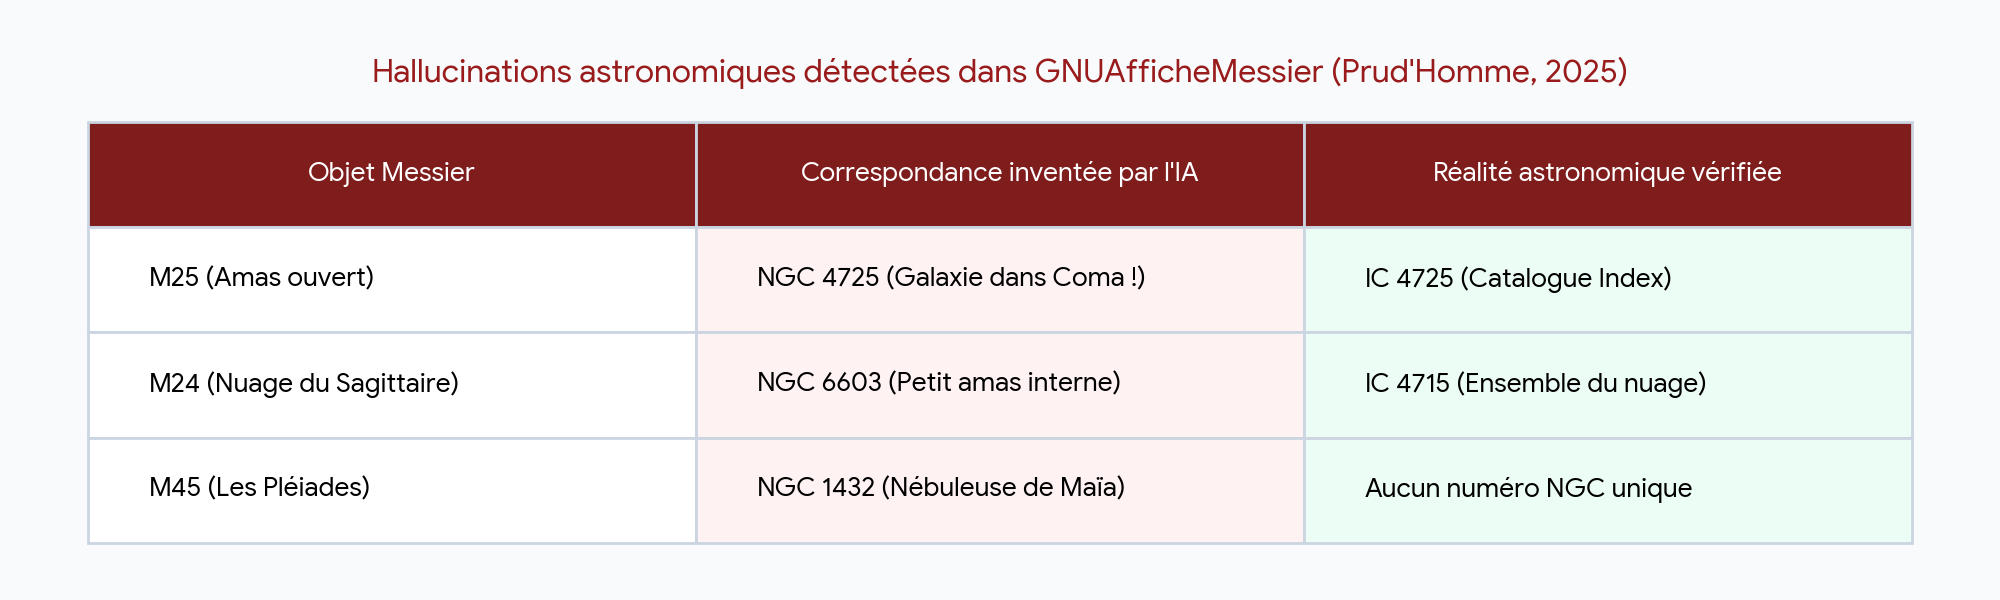
\includegraphics[width=1\linewidth,height=48mm,keepaspectratio]{figures/image11.png}%
\end{column}\end{columns}
\end{frame}
\begin{frame}{Reconnaître une régression}
\vspace{-0.6mm}{\scriptsize\color{SwissMuted}0:32:30 – 0:36 · 3,5 min}\par\smallskip
\begin{columns}[T,onlytextwidth]\begin{column}{.38\textwidth}\raggedright\fontsize{9.6}{12}\selectfont
{\color{SwissAccent}\rule{6mm}{1pt}}\par\medskip
Après une correction, une fonction qui marchait peut cesser de fonctionner.\par\medskip
Rejouez un ancien exemple. Comptez les objets avant et après.\par\medskip
\end{column}\begin{column}{.60\textwidth}\centering
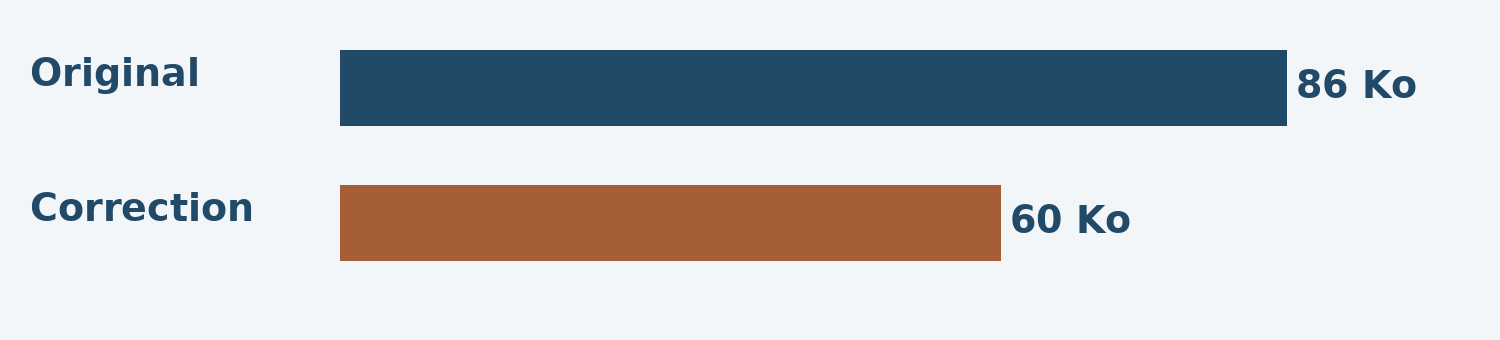
\includegraphics[width=1\linewidth,height=48mm,keepaspectratio]{figures/image12.png}%
\end{column}\end{columns}
\end{frame}
\begin{frame}{Protéger ses fichiers et ses accès}
\vspace{-0.6mm}{\scriptsize\color{SwissMuted}0:36 – 0:39 · 3 min}\par\smallskip
\begin{columns}[T,onlytextwidth]\begin{column}{.38\textwidth}\raggedright\fontsize{9.6}{12}\selectfont
{\color{SwissAccent}\rule{6mm}{1pt}}\par\medskip
Testez sur des copies. Gardez les originaux en lecture seule.\par\medskip
Retirez les clés d'accès des exemples. Vérifiez les droits de réutilisation des images.\par\medskip
\end{column}\begin{column}{.60\textwidth}\centering
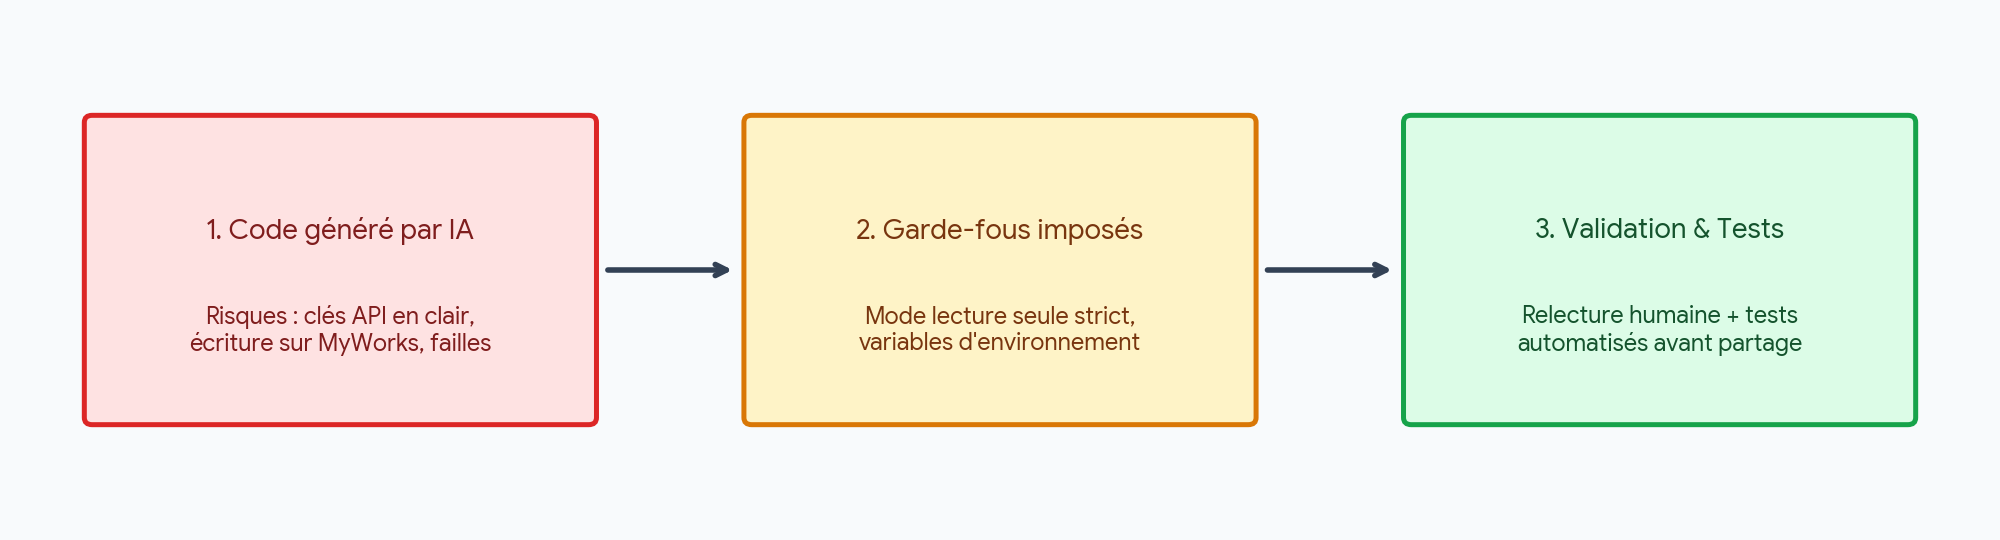
\includegraphics[width=1\linewidth,height=48mm,keepaspectratio]{figures/image13.png}%
\end{column}\end{columns}
\end{frame}
\begin{frame}{Savoir expliquer ce que fait le logiciel}
\vspace{-0.6mm}{\scriptsize\color{SwissMuted}0:39 – 0:42 · 3 min}\par\smallskip
\begin{columns}[T,onlytextwidth]\begin{column}{.38\textwidth}\raggedright\fontsize{9.6}{12}\selectfont
{\color{SwissAccent}\rule{6mm}{1pt}}\par\medskip
Avant de lancer le programme, prédisez sa sortie.\par\medskip
Une cible sous l'horizon apparaît-elle dans la liste? Cherchez quelle règle l'a laissée passer.\par\medskip
\end{column}\begin{column}{.60\textwidth}\centering
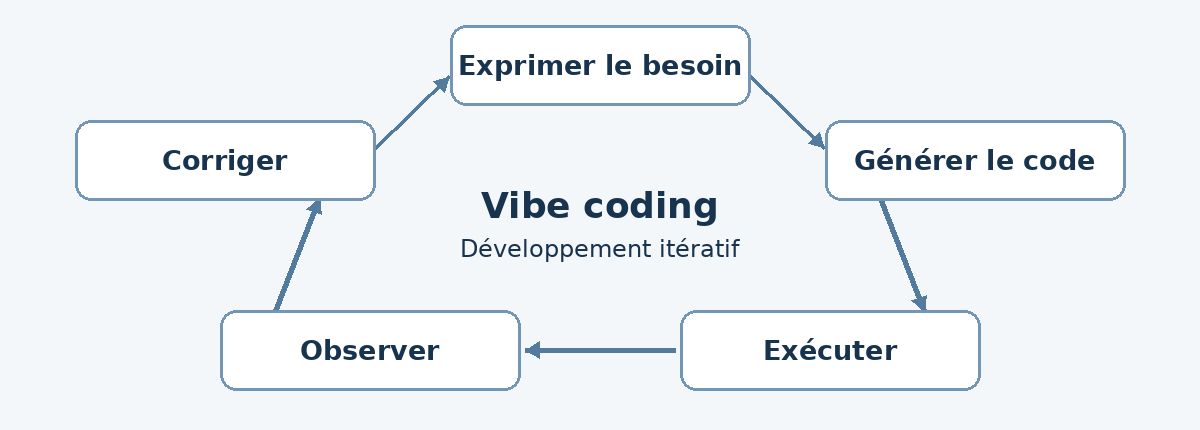
\includegraphics[width=1\linewidth,height=48mm,keepaspectratio]{figures/image14.png}%
\end{column}\end{columns}
\end{frame}
\begin{frame}{Partager le code et les décisions}
\vspace{-0.6mm}{\scriptsize\color{SwissMuted}0:42 – 0:45 · 3 min}\par\smallskip
\begin{columns}[T,onlytextwidth]\begin{column}{.38\textwidth}\raggedright\fontsize{9.6}{12}\selectfont
{\color{SwissAccent}\rule{6mm}{1pt}}\par\medskip
Le logiciel libre met l'accent sur les libertés accordées aux utilisateurs.\par\medskip
L'open source précise des conditions de redistribution. Un projet peut relever des deux approches.\par\medskip
\end{column}\begin{column}{.60\textwidth}\centering
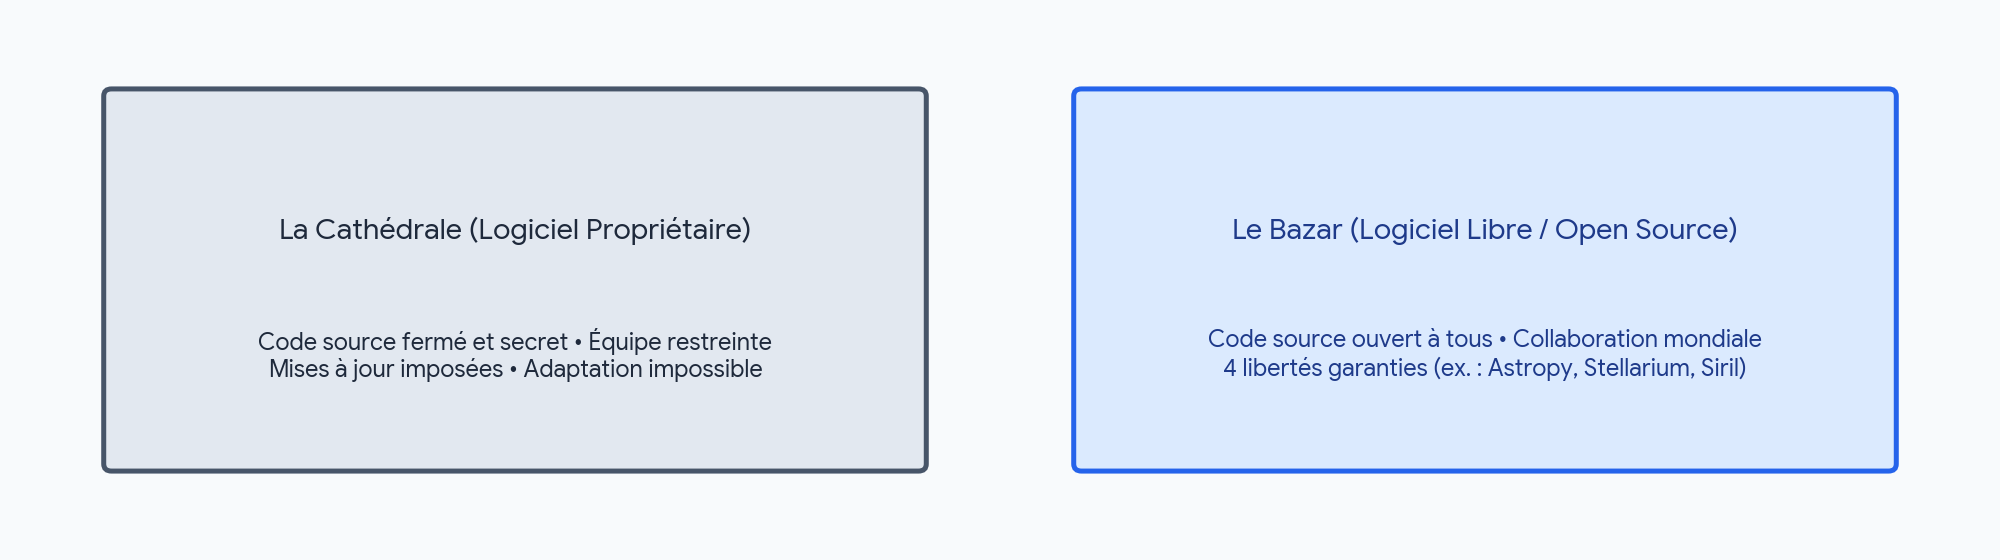
\includegraphics[width=1\linewidth,height=48mm,keepaspectratio]{figures/image15.png}%
\end{column}\end{columns}
\end{frame}
\begin{frame}{Les quatre libertés d'un club}
\vspace{-0.6mm}{\scriptsize\color{SwissMuted}0:45 – 0:48 · 3 min}\par\smallskip
\vfill\large
{\color{SwissAccent}\rule{6mm}{1pt}}\par\medskip
0   Exécuter le programme pour l'usage de son choix.\par\medskip
1   Étudier et modifier son code source.\par\medskip
2   Donner une copie à un autre membre.\par\medskip
3   Partager sa version améliorée.\par\medskip
\vfill
\end{frame}
\begin{frame}{Choisir les conditions de réutilisation}
\vspace{-0.6mm}{\scriptsize\color{SwissMuted}0:48 – 0:51 · 3 min}\par\smallskip
\begin{columns}[T,onlytextwidth]\begin{column}{.38\textwidth}\raggedright\fontsize{9.6}{12}\selectfont
{\color{SwissAccent}\rule{6mm}{1pt}}\par\medskip
MIT et BSD permettent une réutilisation étendue avec conservation des mentions requises.\par\medskip
La GPL demande de préserver des libertés lors de la redistribution d'une version couverte.\par\medskip
\end{column}\begin{column}{.60\textwidth}\centering
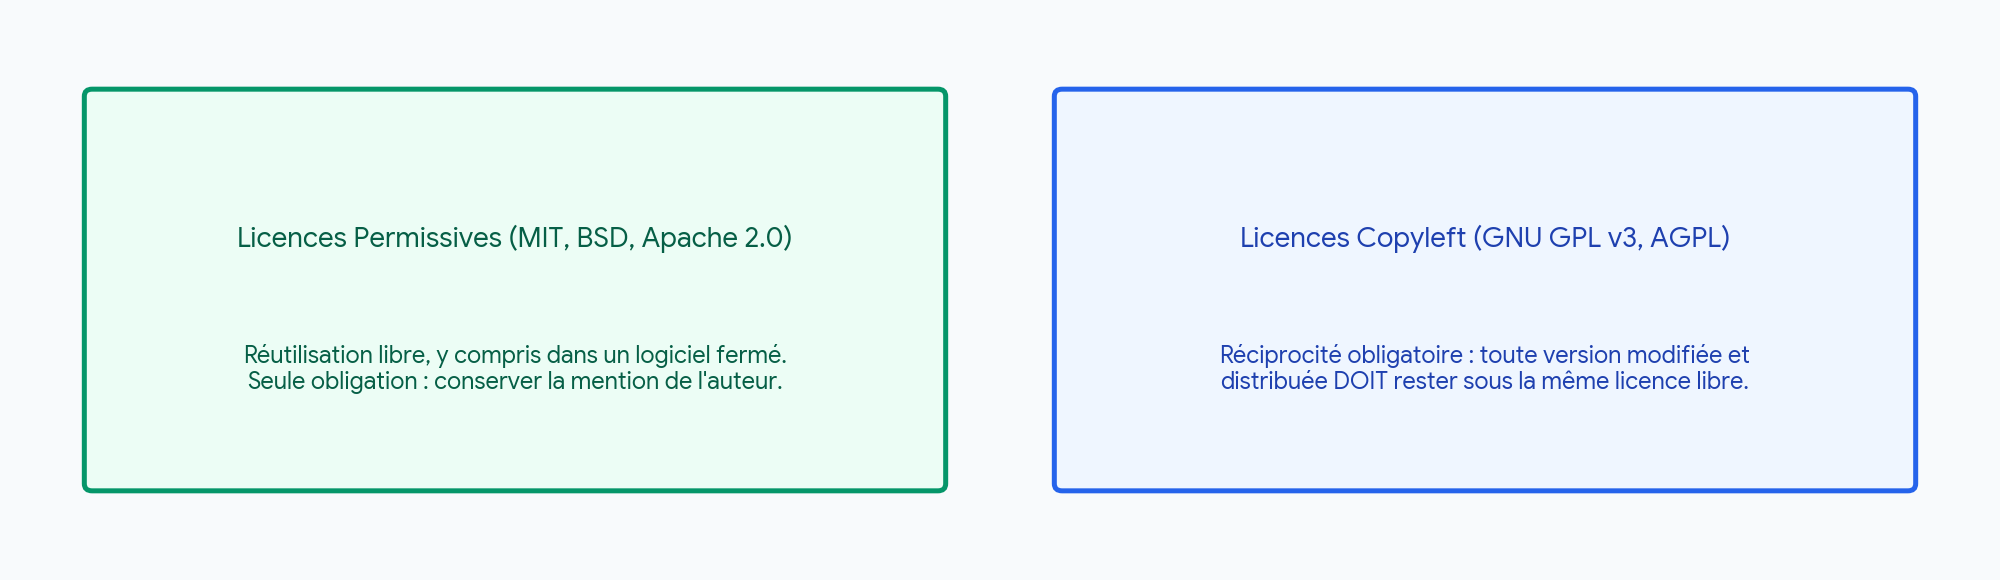
\includegraphics[width=1\linewidth,height=48mm,keepaspectratio]{figures/image16.png}%
\end{column}\end{columns}
\end{frame}
\begin{frame}{Qui fait vivre un projet libre?}
\vspace{-0.6mm}{\scriptsize\color{SwissMuted}0:51 – 0:53 · 2 min}\par\smallskip
\begin{columns}[T,onlytextwidth]\begin{column}{.38\textwidth}\raggedright\fontsize{9.6}{12}\selectfont
{\color{SwissAccent}\rule{6mm}{1pt}}\par\medskip
Certains outils dépendent d'une seule personne. D'autres réunissent de nombreux contributeurs.\par\medskip
Avant d'adopter un outil, repérez qui le maintient et comment demander de l'aide.\par\medskip
\end{column}\begin{column}{.60\textwidth}\centering
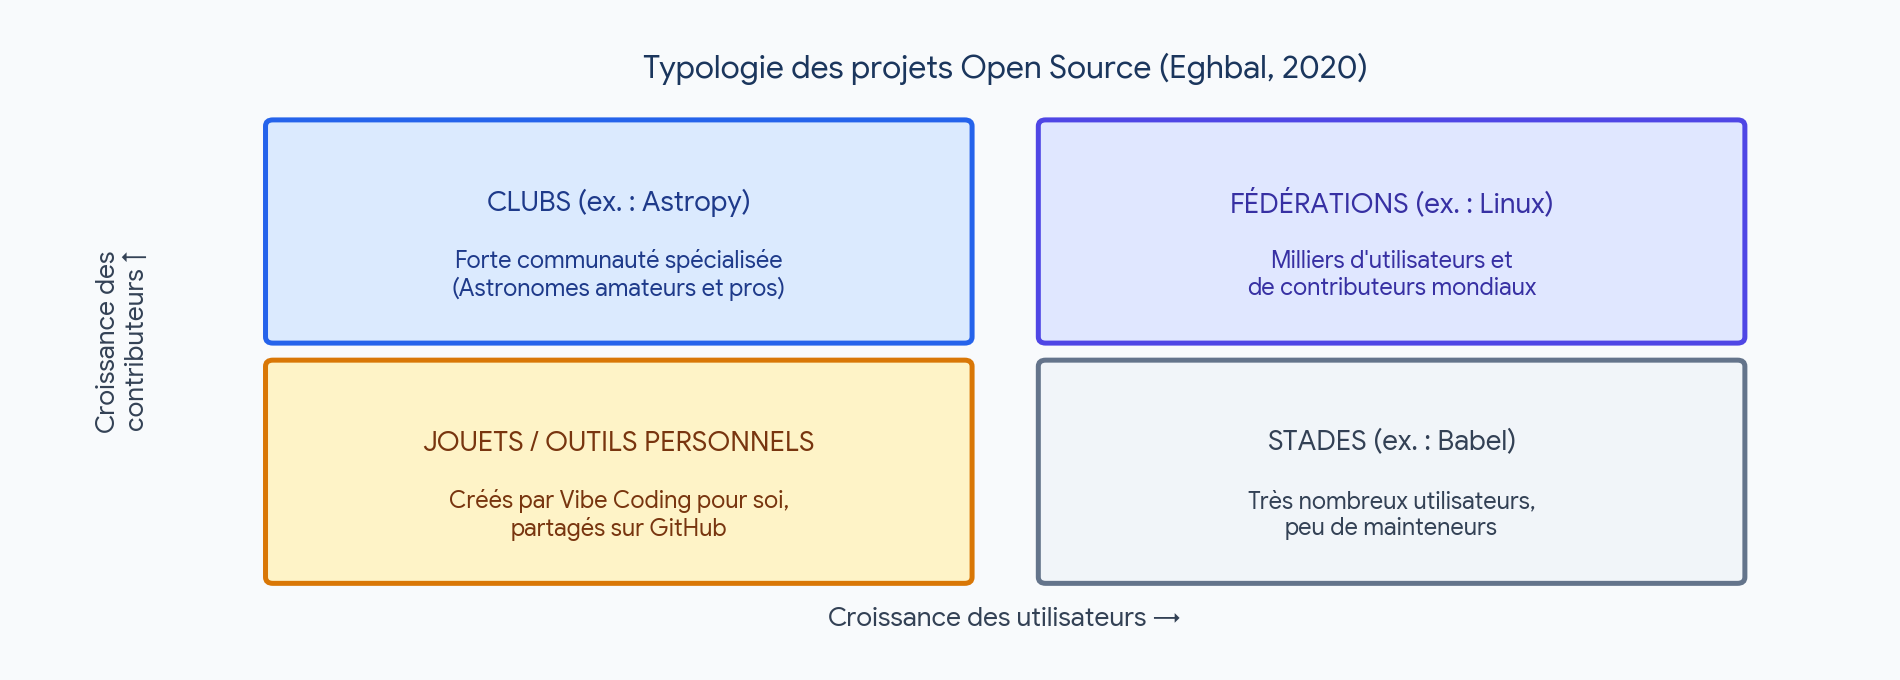
\includegraphics[width=1\linewidth,height=48mm,keepaspectratio]{figures/image17.png}%
\end{column}\end{columns}
\end{frame}
\begin{frame}{Un prompt est une consigne}
\vspace{-0.6mm}{\scriptsize\color{SwissMuted}0:53 – 0:55:30 · 2,5 min}\par\smallskip
\begin{columns}[T,onlytextwidth]\begin{column}{.38\textwidth}\raggedright\fontsize{9.6}{12}\selectfont
{\color{SwissAccent}\rule{6mm}{1pt}}\par\medskip
« Trie mes images » laisse plusieurs décisions ouvertes.\par\medskip
Précisez le dossier, la règle de tri et la forme du résultat attendu.\par\medskip
\end{column}\begin{column}{.60\textwidth}\centering
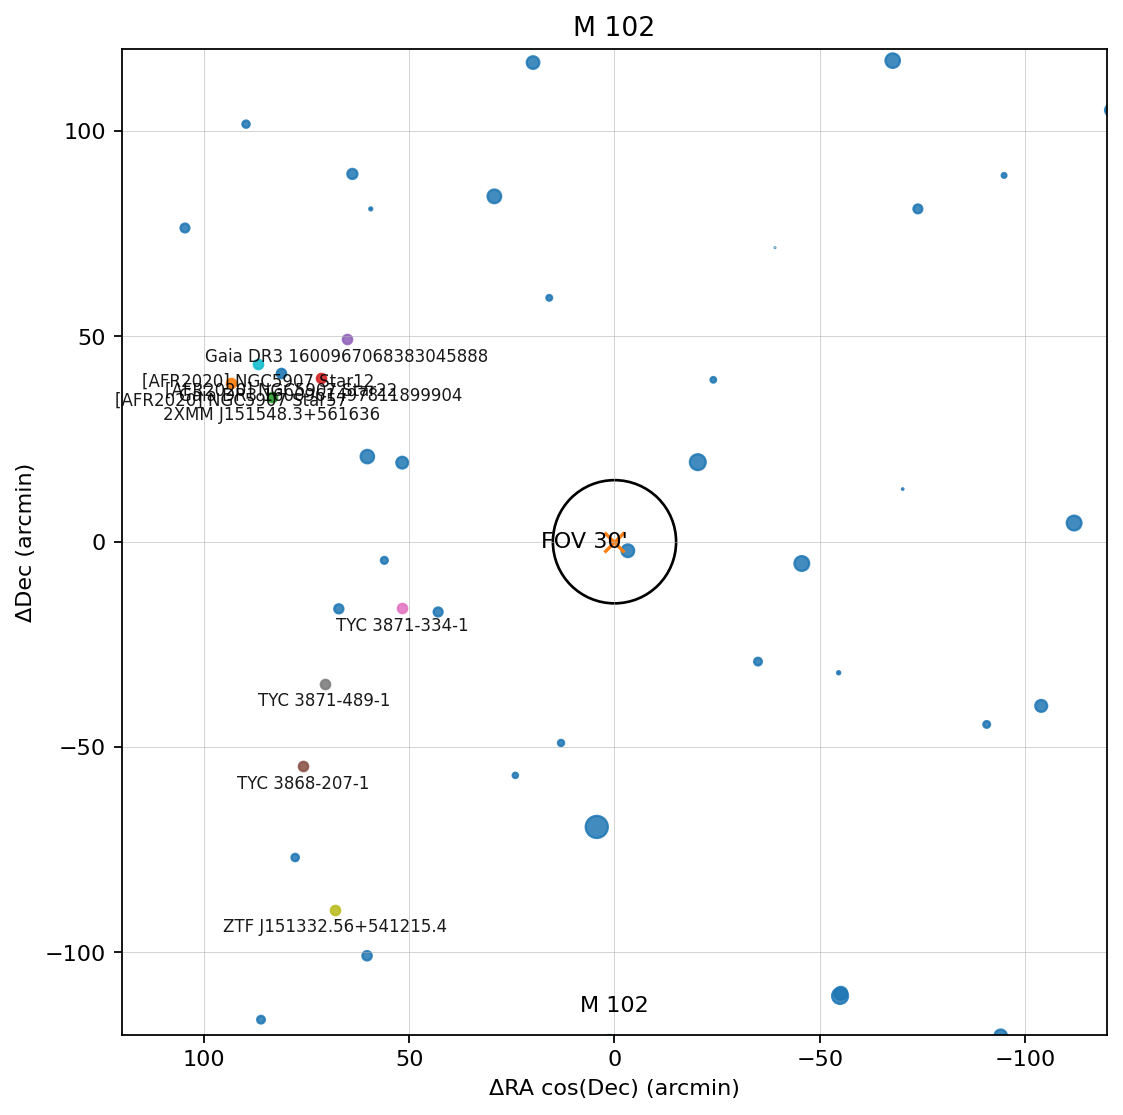
\includegraphics[width=1\linewidth,height=48mm,keepaspectratio]{figures/image18.png}%
\end{column}\end{columns}
\end{frame}
\begin{frame}{Écrire une consigne que l'on peut tester}
\vspace{-0.6mm}{\scriptsize\color{SwissMuted}0:55:30 – 0:58:30 · 3 min}\par\smallskip
\begin{columns}[T,onlytextwidth]\begin{column}{.38\textwidth}\raggedright\fontsize{9.6}{12}\selectfont
{\color{SwissAccent}\rule{6mm}{1pt}}\par\medskip
Donnez le rôle, le contexte, la tâche, les contraintes et le résultat attendu.\par\medskip
« Lis ces copies FITS. Produis un tableau objet, date et durée. Signale les champs absents. »\par\medskip
\end{column}\begin{column}{.60\textwidth}\centering
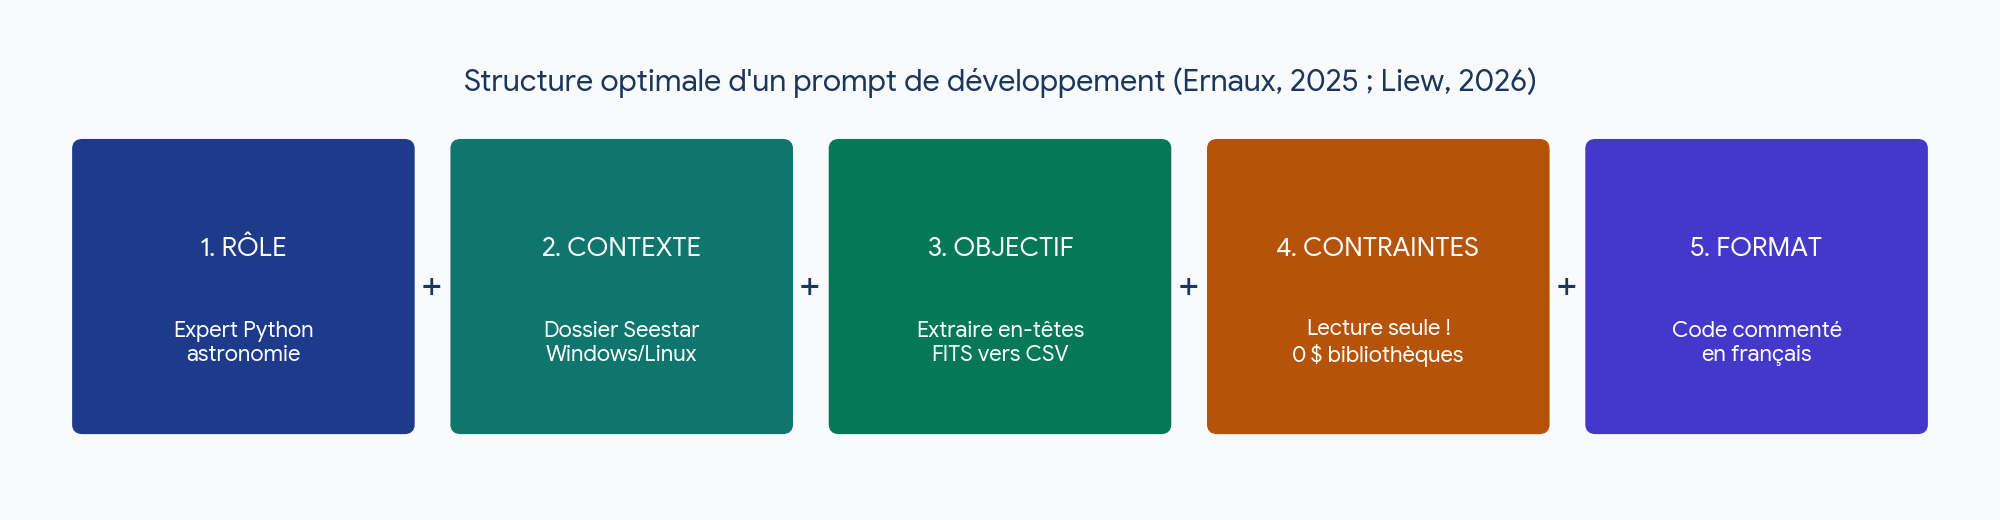
\includegraphics[width=1\linewidth,height=48mm,keepaspectratio]{figures/image19.png}%
\end{column}\end{columns}
\end{frame}
\begin{frame}{Cinq façons de préciser une demande}
\vspace{-0.6mm}{\scriptsize\color{SwissMuted}0:58:30 – 1:02 · 3,5 min}\par\smallskip
\vfill\large
{\color{SwissAccent}\rule{6mm}{1pt}}\par\medskip
Montrez deux exemples de fichiers. Demandez un plan court.\par\medskip
Invitez l'IA à poser ses questions. Faites-lui relire sa proposition.\par\medskip
Demandez-lui ensuite de reformuler la consigne.\par\medskip
\vfill
\end{frame}
\begin{frame}{Remplacer les demandes vagues}
\vspace{-0.6mm}{\scriptsize\color{SwissMuted}1:02 – 1:04:30 · 2,5 min}\par\smallskip
\vfill\large
{\color{SwissAccent}\rule{6mm}{1pt}}\par\medskip
« Corrige ça » \(\rightarrow\) nommez le fichier et décrivez le problème.\par\medskip
« Améliore tout » \(\rightarrow\) choisissez une modification.\par\medskip
« Rends-le plus beau » \(\rightarrow\) donnez un critère visible.\par\medskip
\vfill
\end{frame}
\begin{frame}{Chat, Work et Codex en pratique}
\vspace{-0.6mm}{\scriptsize\color{SwissMuted}1:04:30 – 1:09 · 4,5 min}\par\smallskip
\begin{columns}[T,onlytextwidth]\begin{column}{.38\textwidth}\raggedright\fontsize{9.6}{12}\selectfont
{\color{SwissAccent}\rule{6mm}{1pt}}\par\medskip
Chat pour discuter d'une idée. Work pour produire un document à partir de fichiers.\par\medskip
Codex pour modifier un projet et lancer ses tests dans un environnement autorisé.\par\medskip
\end{column}\begin{column}{.60\textwidth}\centering
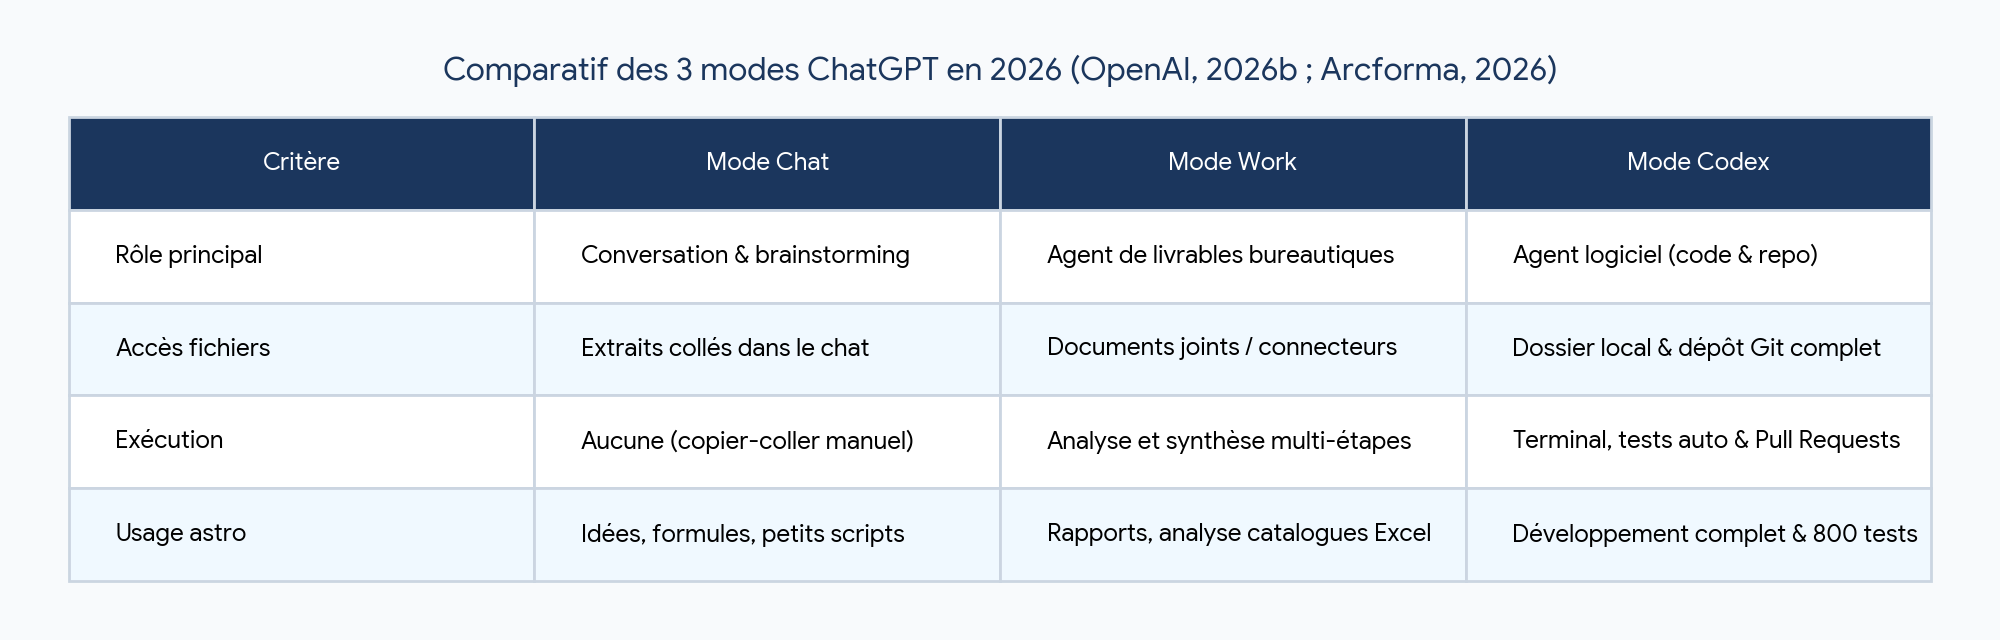
\includegraphics[width=1\linewidth,height=48mm,keepaspectratio]{figures/image20.png}%
\end{column}\end{columns}
\end{frame}
\begin{frame}{Comprendre le coût d'une requête}
\vspace{-0.6mm}{\scriptsize\color{SwissMuted}1:09 – 1:13 · 4 min}\par\smallskip
\begin{columns}[T,onlytextwidth]\begin{column}{.38\textwidth}\raggedright\fontsize{9.6}{12}\selectfont
{\color{SwissAccent}\rule{6mm}{1pt}}\par\medskip
Un token est un fragment de texte traité par le modèle.\par\medskip
Distinguez entrée, entrée mise en cache et sortie. Multipliez chaque volume par son tarif.\par\medskip
Les chiffres de la figure illustrent le document source. Vérifiez le forfait avant de chiffrer un projet.\par\medskip
\end{column}\begin{column}{.60\textwidth}\centering
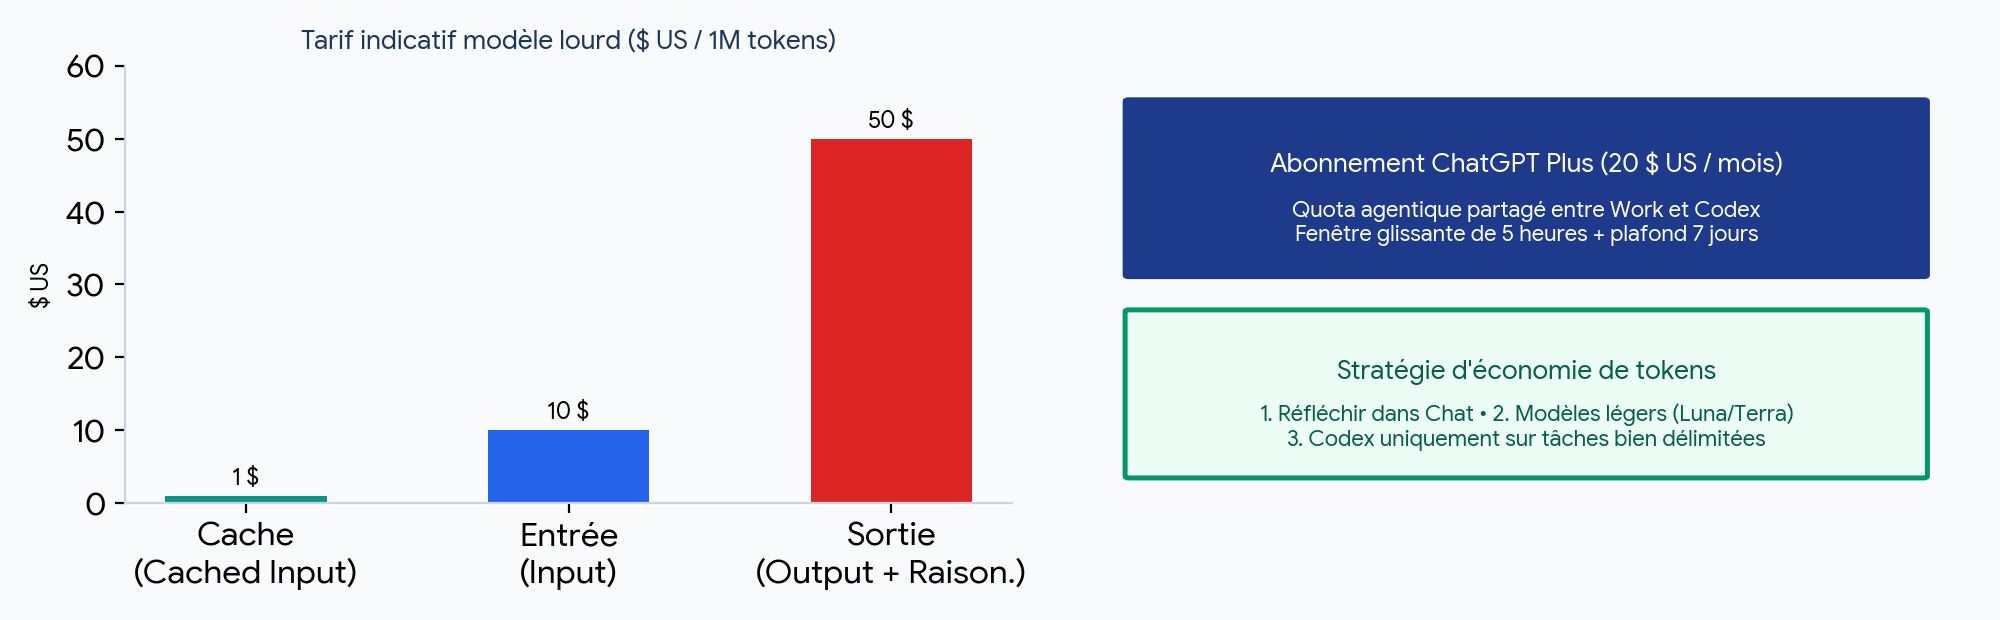
\includegraphics[width=1\linewidth,height=48mm,keepaspectratio]{figures/image21.png}%
\end{column}\end{columns}
\end{frame}
\begin{frame}{Se repérer dans un dépôt}
\vspace{-0.6mm}{\scriptsize\color{SwissMuted}1:13 – 1:17 · 4 min}\par\smallskip
\vfill\large
{\color{SwissAccent}\rule{6mm}{1pt}}\par\medskip
src/ contient le code. tests/ contient les essais reproductibles.\par\medskip
docs/ explique le projet. README.md présente le premier essai.\par\medskip
.gitignore indique quels fichiers générés ou volumineux laisser hors du dépôt.\par\medskip
\vfill
\end{frame}
\begin{frame}{Cinq fichiers pour travailler ensemble}
\vspace{-0.6mm}{\scriptsize\color{SwissMuted}1:17 – 1:23 · 6 min}\par\smallskip
\vfill\large
{\color{SwissAccent}\rule{6mm}{1pt}}\par\medskip
README.md explique comment commencer. CHANGELOG.md décrit les changements.\par\medskip
ROADMAP.md annonce les prochaines étapes. CONTRIBUTING.md explique comment participer.\par\medskip
AGENTS.md précise les consignes données à l'assistant.\par\medskip
\vfill
\end{frame}
\begin{frame}{Git conserve l'historique du projet}
\vspace{-0.6mm}{\scriptsize\color{SwissMuted}1:23 – 1:26 · 3 min}\par\smallskip
\vfill\large
{\color{SwissAccent}\rule{6mm}{1pt}}\par\medskip
Git enregistre vos versions sur votre ordinateur.\par\medskip
GitHub héberge une copie du dépôt et permet au club de proposer des changements.\par\medskip
\vfill
\end{frame}
\begin{frame}{Enregistrer un changement avec Git}
\vspace{-0.6mm}{\scriptsize\color{SwissMuted}1:26 – 1:30 · 4 min}\par\smallskip
\begin{columns}[T,onlytextwidth]\begin{column}{.38\textwidth}\raggedright\fontsize{9.6}{12}\selectfont
{\color{SwissAccent}\rule{6mm}{1pt}}\par\medskip
git status — repérer les fichiers modifiés.\par\medskip
git add README.md — choisir le fichier.\par\medskip
git commit -m "Documenter le premier essai" — enregistrer cette étape.\par\medskip
\end{column}\begin{column}{.60\textwidth}\centering
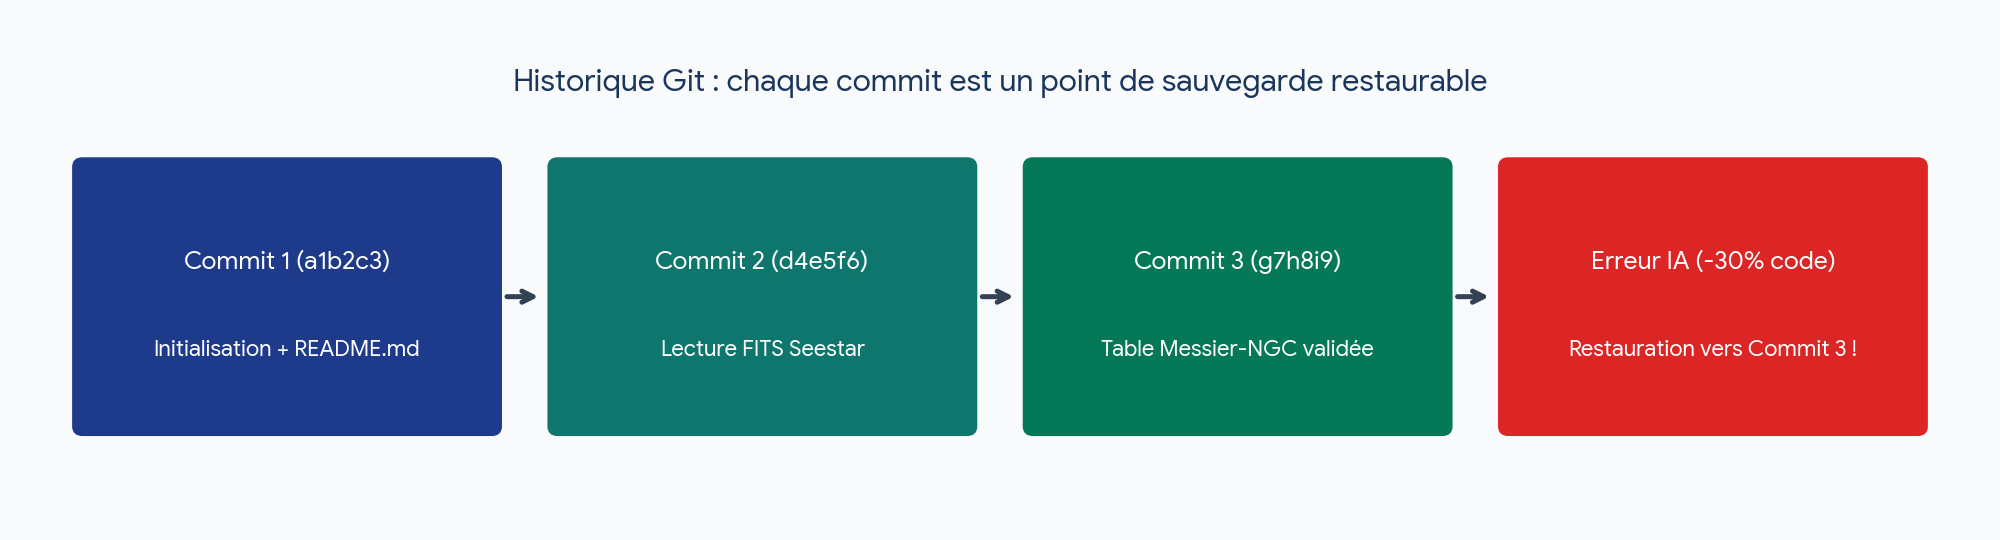
\includegraphics[width=1\linewidth,height=48mm,keepaspectratio]{figures/image22.png}%
\end{column}\end{columns}
\end{frame}
\begin{frame}{Essayer une idée sur une branche}
\vspace{-0.6mm}{\scriptsize\color{SwissMuted}1:30 – 1:33:30 · 3,5 min}\par\smallskip
\begin{columns}[T,onlytextwidth]\begin{column}{.38\textwidth}\raggedright\fontsize{9.6}{12}\selectfont
{\color{SwissAccent}\rule{6mm}{1pt}}\par\medskip
Une branche garde une modification à part pendant son essai.\par\medskip
Faites un commit après chaque étape vérifiée. Intégrez la branche quand le résultat convient.\par\medskip
\end{column}\begin{column}{.60\textwidth}\centering
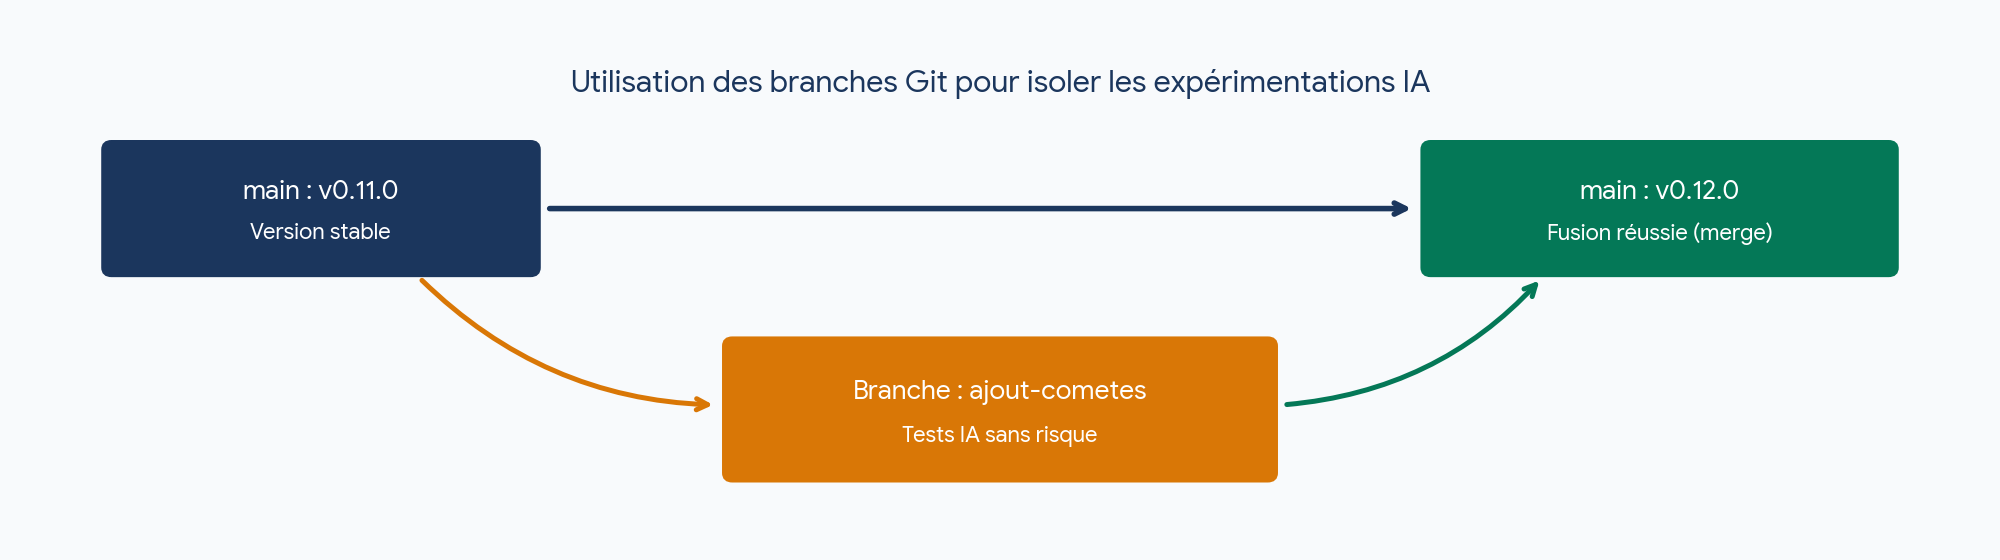
\includegraphics[width=1\linewidth,height=48mm,keepaspectratio]{figures/image23.png}%
\end{column}\end{columns}
\end{frame}
\begin{frame}{Lire un numéro de version}
\vspace{-0.6mm}{\scriptsize\color{SwissMuted}1:33:30 – 1:37 · 3,5 min}\par\smallskip
\begin{columns}[T,onlytextwidth]\begin{column}{.38\textwidth}\raggedright\fontsize{9.6}{12}\selectfont
{\color{SwissAccent}\rule{6mm}{1pt}}\par\medskip
MAJEUR.MINEUR.CORRECTIF indique l'effet d'un changement sur l'interface publique.\par\medskip
Après 1.2.0, une correction compatible donne 1.2.1. Une fonction compatible donne 1.3.0.\par\medskip
\end{column}\begin{column}{.60\textwidth}\centering
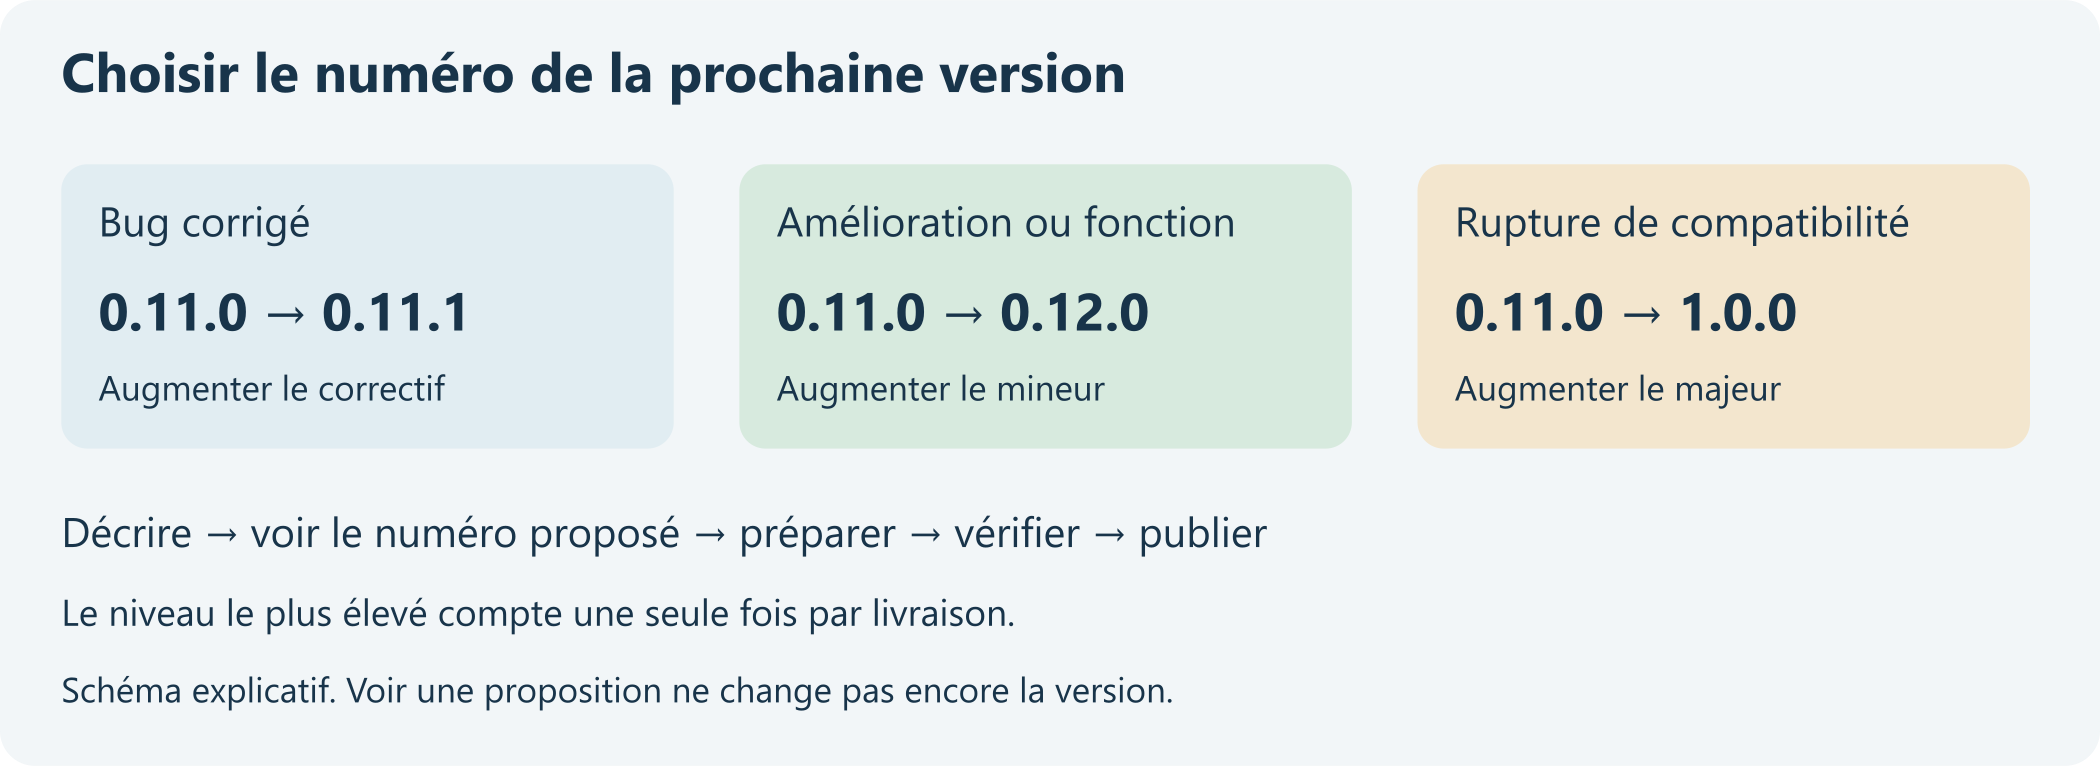
\includegraphics[width=1\linewidth,height=48mm,keepaspectratio]{figures/image24.png}%
\end{column}\end{columns}
\end{frame}
\begin{frame}{Quatre projets issus du terrain}
\vspace{-0.6mm}{\scriptsize\color{SwissMuted}1:37 – 1:39 · 2 min}\par\smallskip
\vfill\large
{\color{SwissAccent}\rule{6mm}{1pt}}\par\medskip
GNU Affiche Messier transforme une collection en affiche.\par\medskip
GNU Astro Galery documente les images. GNU Astrolist prépare une soirée.\par\medskip
GNU Astrophotography Recycle réutilise des poses archivées.\par\medskip
\vfill
\end{frame}
\begin{frame}{Une affiche pour suivre ses objets Messier}
\vspace{-0.6mm}{\scriptsize\color{SwissMuted}1:39 – 1:41:30 · 2,5 min}\par\smallskip
\begin{columns}[T,onlytextwidth]\begin{column}{.38\textwidth}\raggedright\fontsize{9.6}{12}\selectfont
{\color{SwissAccent}\rule{6mm}{1pt}}\par\medskip
110 emplacements sur une affiche de 24 \(\times\) 36 po.\par\medskip
M31 et NGC 224 désignent la même galaxie. Comptez-la une seule fois.\par\medskip
\end{column}\begin{column}{.60\textwidth}\centering
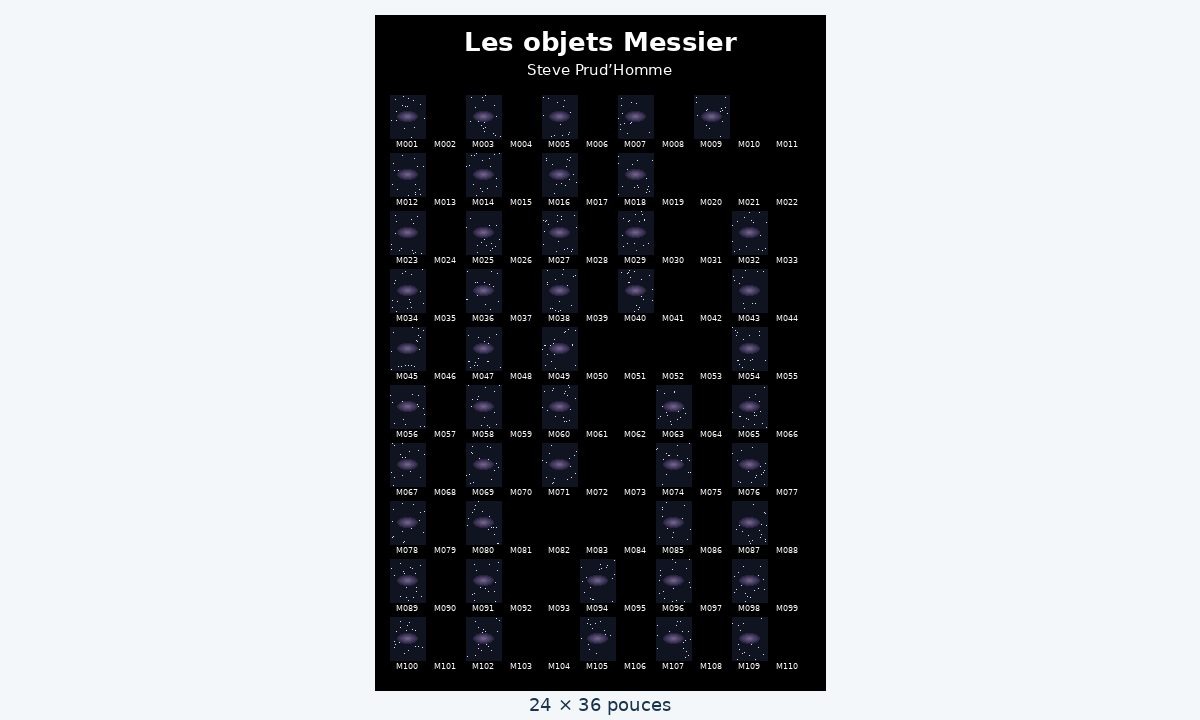
\includegraphics[width=.49\linewidth,height=24mm,keepaspectratio]{figures/image25.png}%
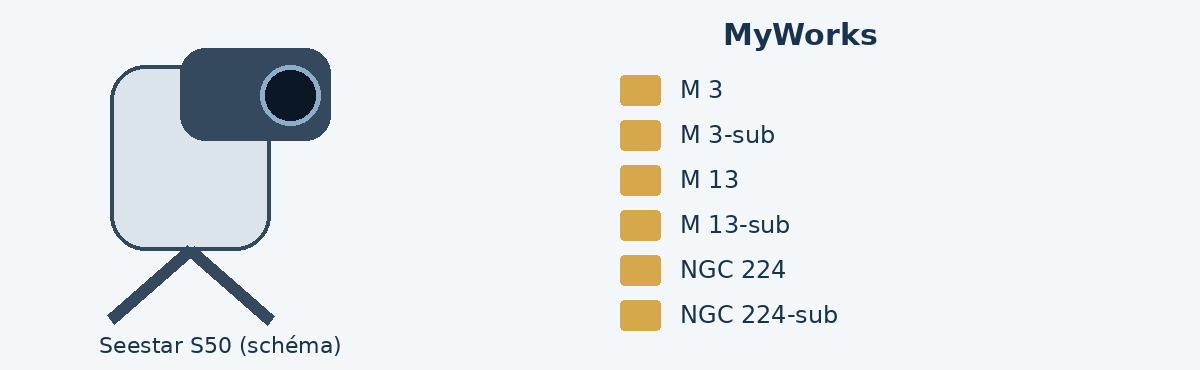
\includegraphics[width=.49\linewidth,height=24mm,keepaspectratio]{figures/image26.png}\par

\includegraphics[width=.49\linewidth,height=24mm,keepaspectratio]{figures/image27.png}%
\end{column}\end{columns}
\end{frame}
\begin{frame}{Du premier échange au premier essai}
\vspace{-0.6mm}{\scriptsize\color{SwissMuted}1:41:30 – 1:44:30 · 3 min}\par\smallskip
\begin{columns}[T,onlytextwidth]\begin{column}{.38\textwidth}\raggedright\fontsize{9.6}{12}\selectfont
{\color{SwissAccent}\rule{6mm}{1pt}}\par\medskip
Le programme parcourt le dossier MyWorks du Seestar.\par\medskip
Premier essai documenté : 35 objets Messier sur 110. Comparez la liste aux dossiers sources.\par\medskip
\end{column}\begin{column}{.60\textwidth}\centering

\includegraphics[width=.49\linewidth,height=35mm,keepaspectratio]{figures/image28.png}%
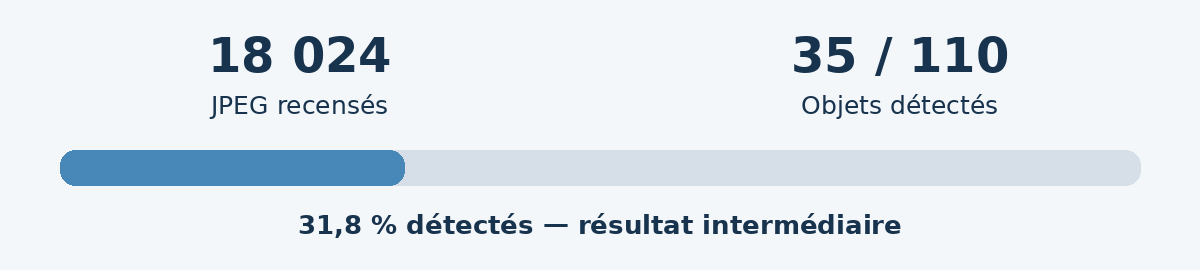
\includegraphics[width=.49\linewidth,height=35mm,keepaspectratio]{figures/image29.png}\par
\end{column}\end{columns}
\end{frame}
\begin{frame}{Du fichier FITS à la galerie Web}
\vspace{-0.6mm}{\scriptsize\color{SwissMuted}1:44:30 – 1:49 · 4,5 min}\par\smallskip
\begin{columns}[T,onlytextwidth]\begin{column}{.38\textwidth}\raggedright\fontsize{9.6}{12}\selectfont
{\color{SwissAccent}\rule{6mm}{1pt}}\par\medskip
Suivez M44 du dossier d'observation à sa fiche.\par\medskip
Repérez la durée de pose et la date dans l'en-tête. La carte aide à situer le champ.\par\medskip
\end{column}\begin{column}{.60\textwidth}\centering
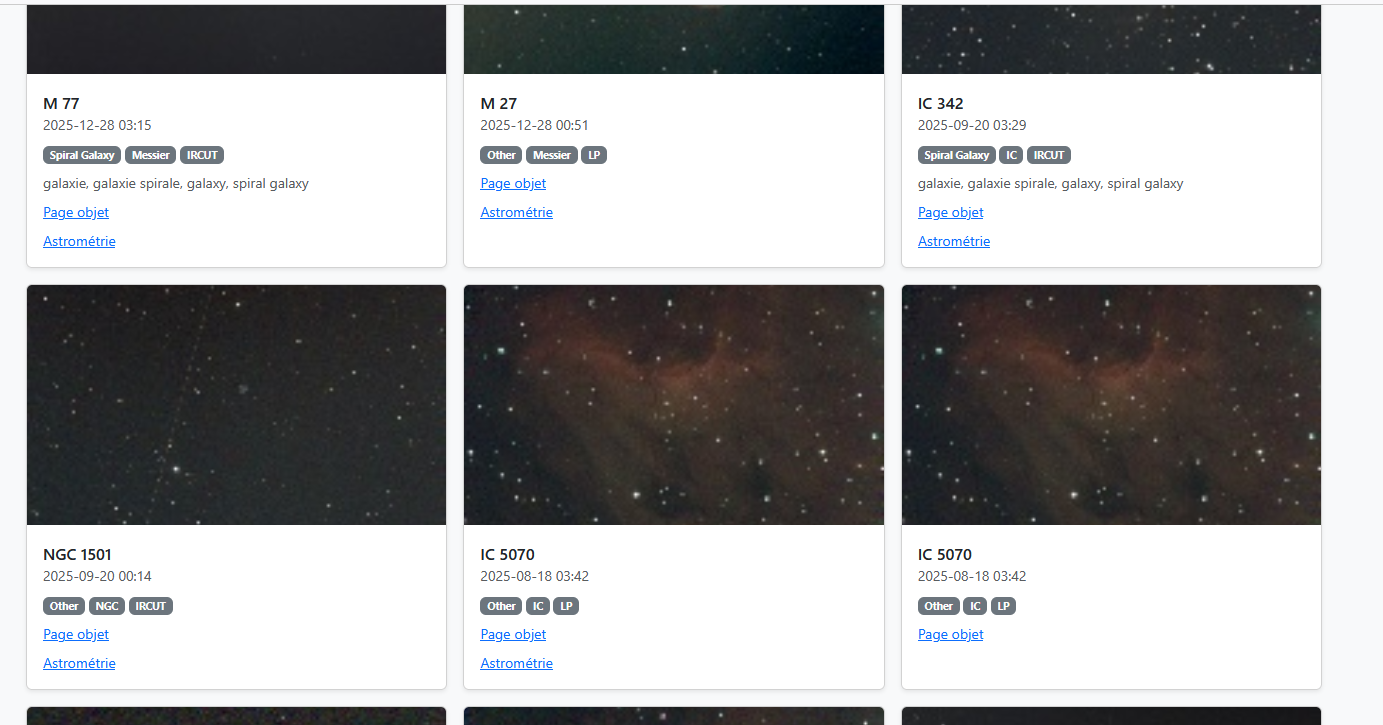
\includegraphics[width=.49\linewidth,height=24mm,keepaspectratio]{figures/image30.png}%
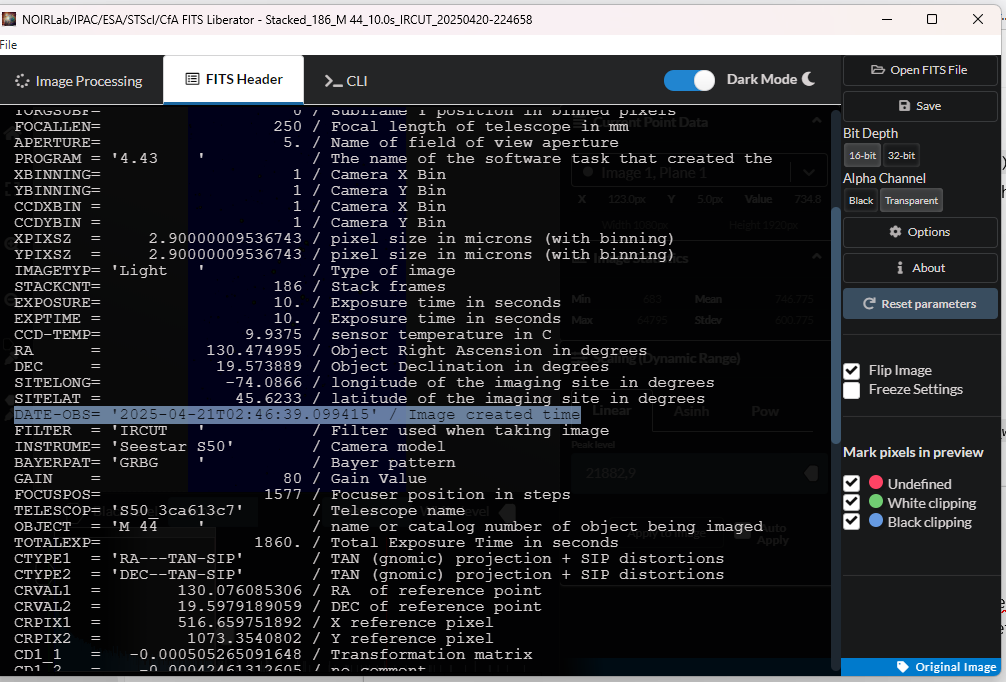
\includegraphics[width=.49\linewidth,height=24mm,keepaspectratio]{figures/image31.png}\par
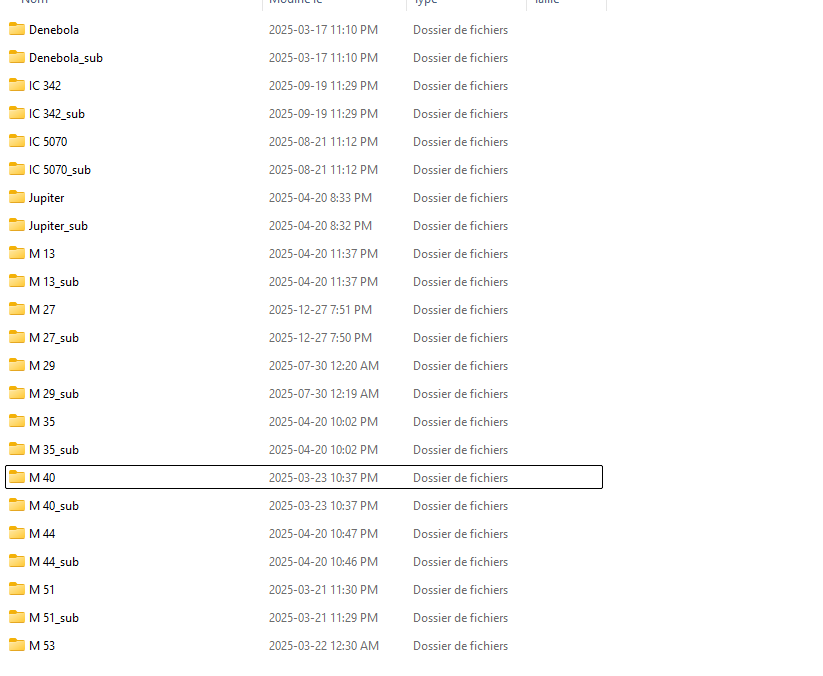
\includegraphics[width=.49\linewidth,height=24mm,keepaspectratio]{figures/image32.png}%
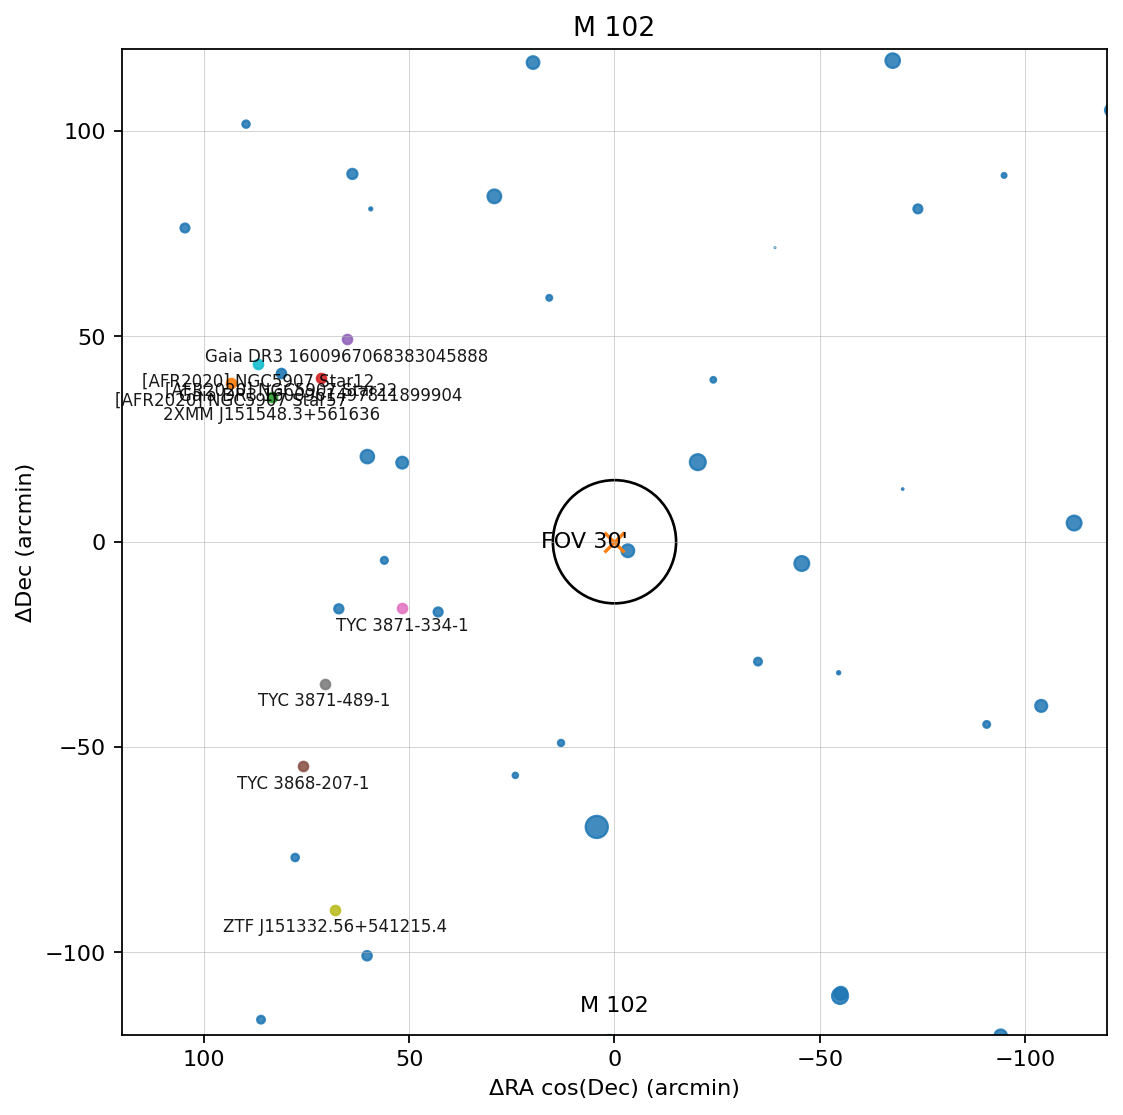
\includegraphics[width=.49\linewidth,height=24mm,keepaspectratio]{figures/image18.png}\par
\end{column}\end{columns}
\end{frame}
\begin{frame}{Préparer une soirée avec GNU Astrolist}
\vspace{-0.6mm}{\scriptsize\color{SwissMuted}1:49 – 1:53:30 · 4,5 min}\par\smallskip
\begin{columns}[T,onlytextwidth]\begin{column}{.38\textwidth}\raggedright\fontsize{9.6}{12}\selectfont
{\color{SwissAccent}\rule{6mm}{1pt}}\par\medskip
Choisissez une plage de hauteurs visible depuis votre site.\par\medskip
Comparez la sélection au rapport PDF. Consultez les acquisitions passées en lecture seule.\par\medskip
\end{column}\begin{column}{.60\textwidth}\centering
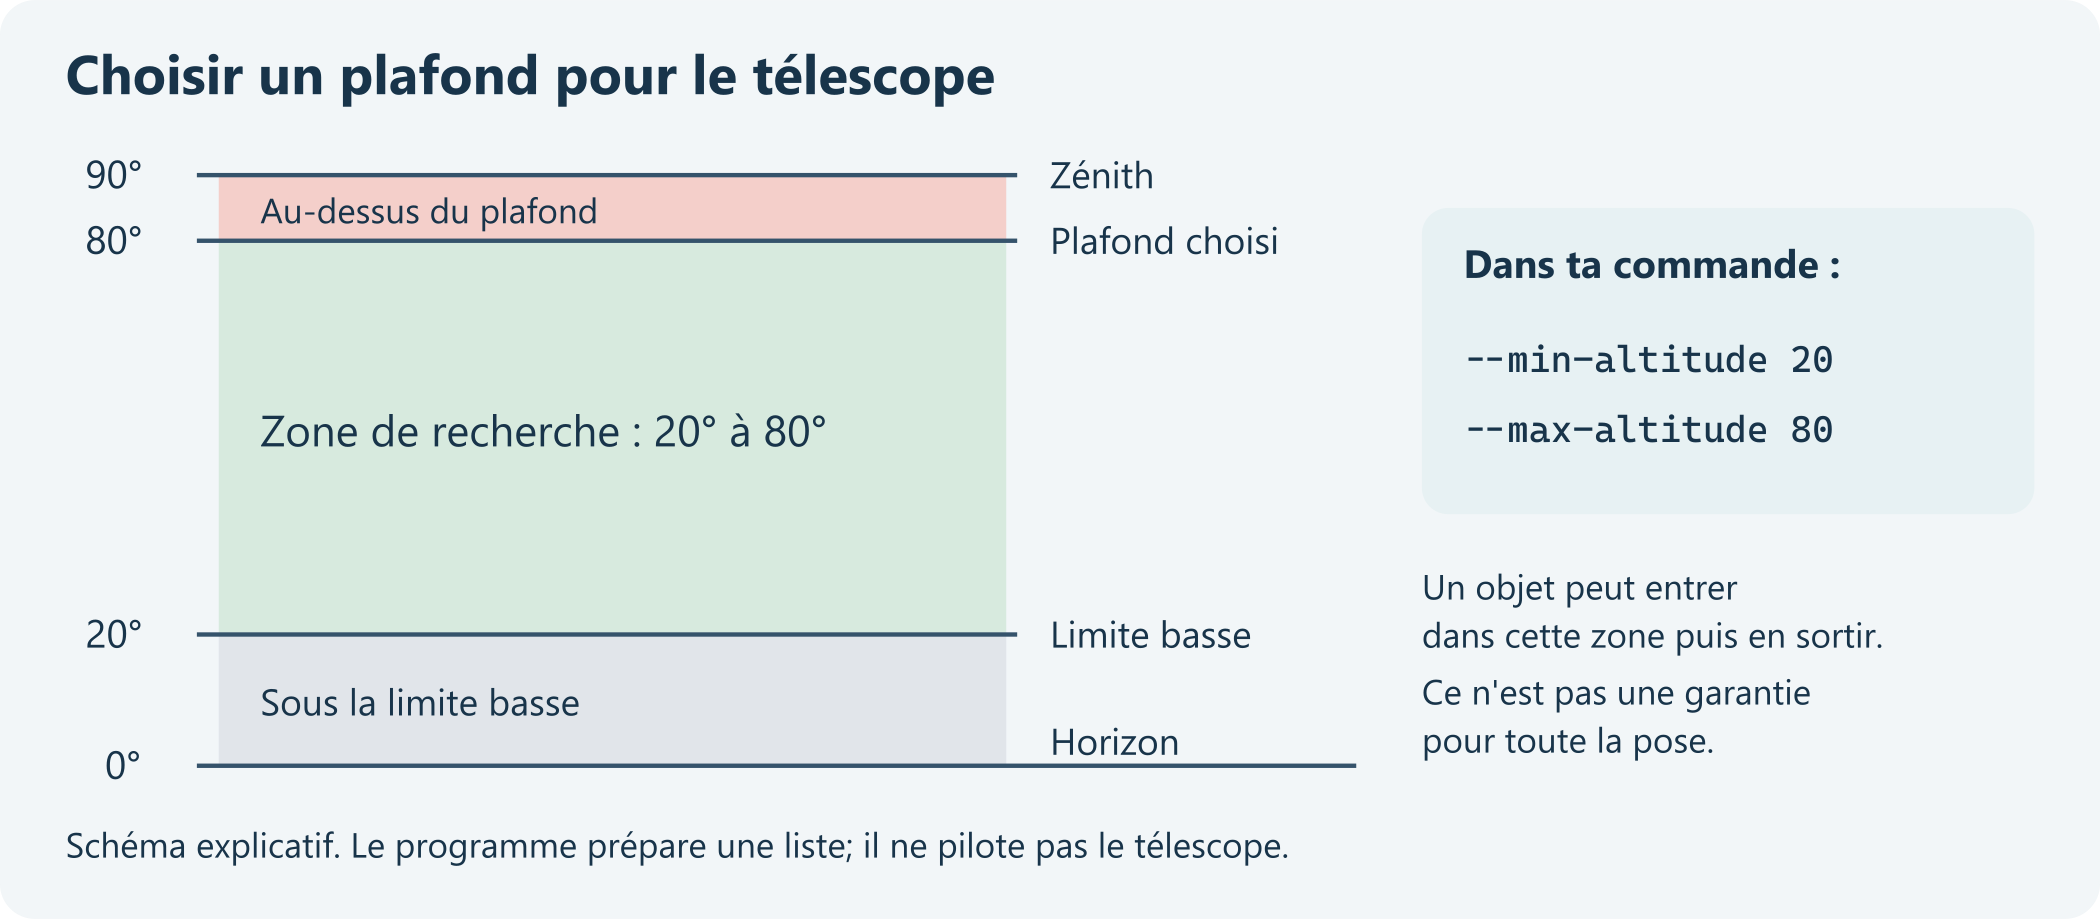
\includegraphics[width=.49\linewidth,height=24mm,keepaspectratio]{figures/image33.png}%
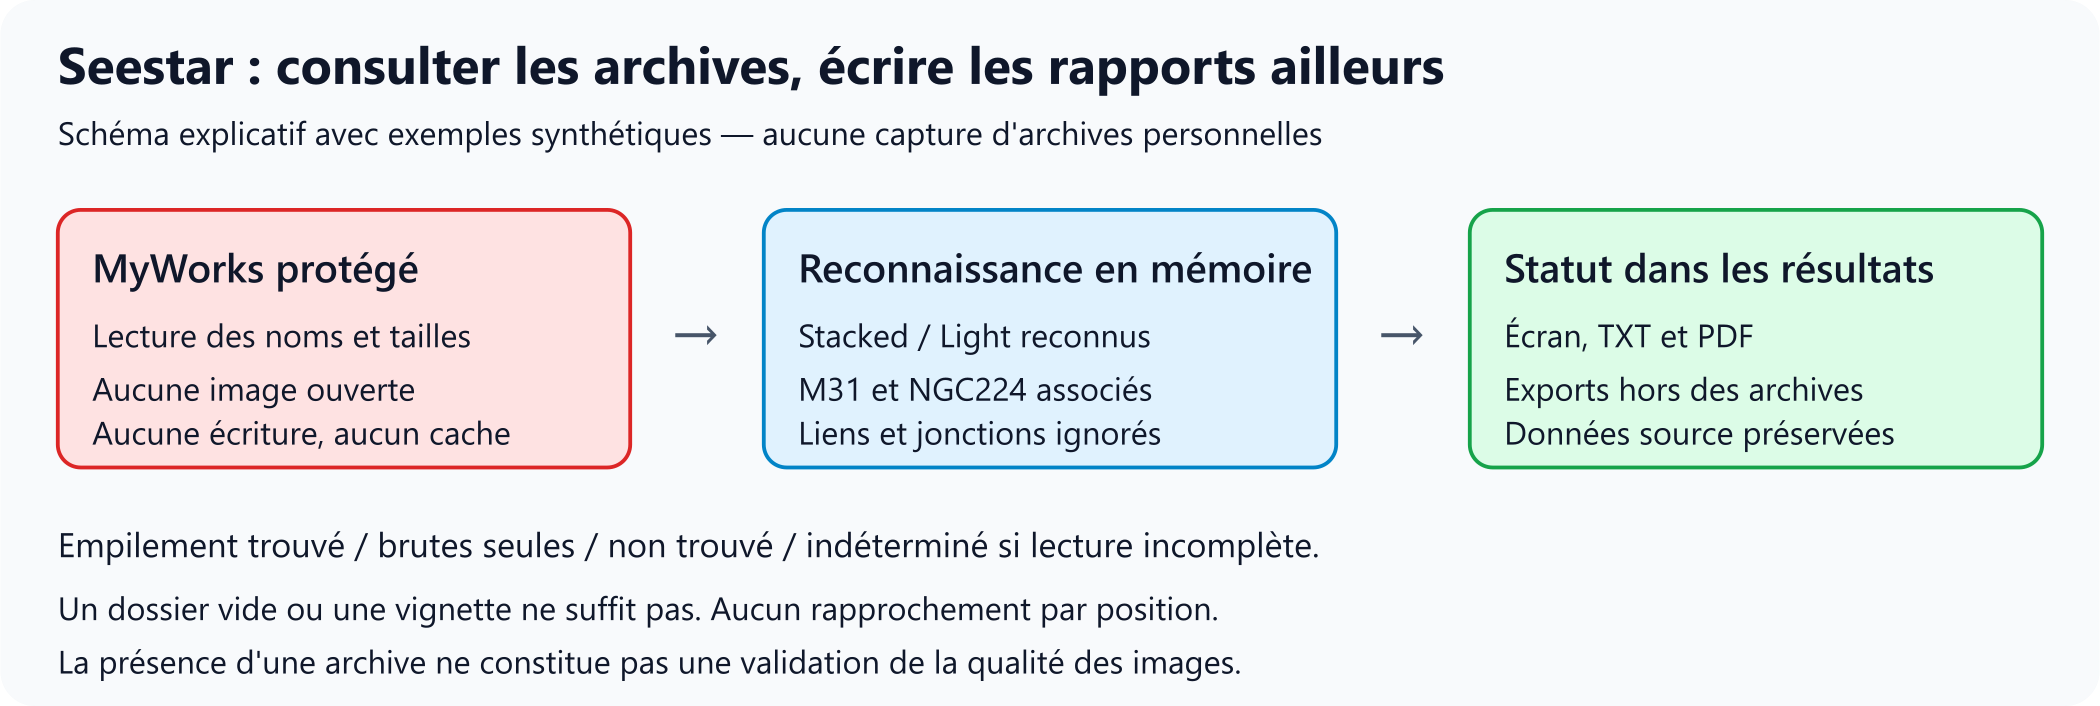
\includegraphics[width=.49\linewidth,height=24mm,keepaspectratio]{figures/image34.png}\par
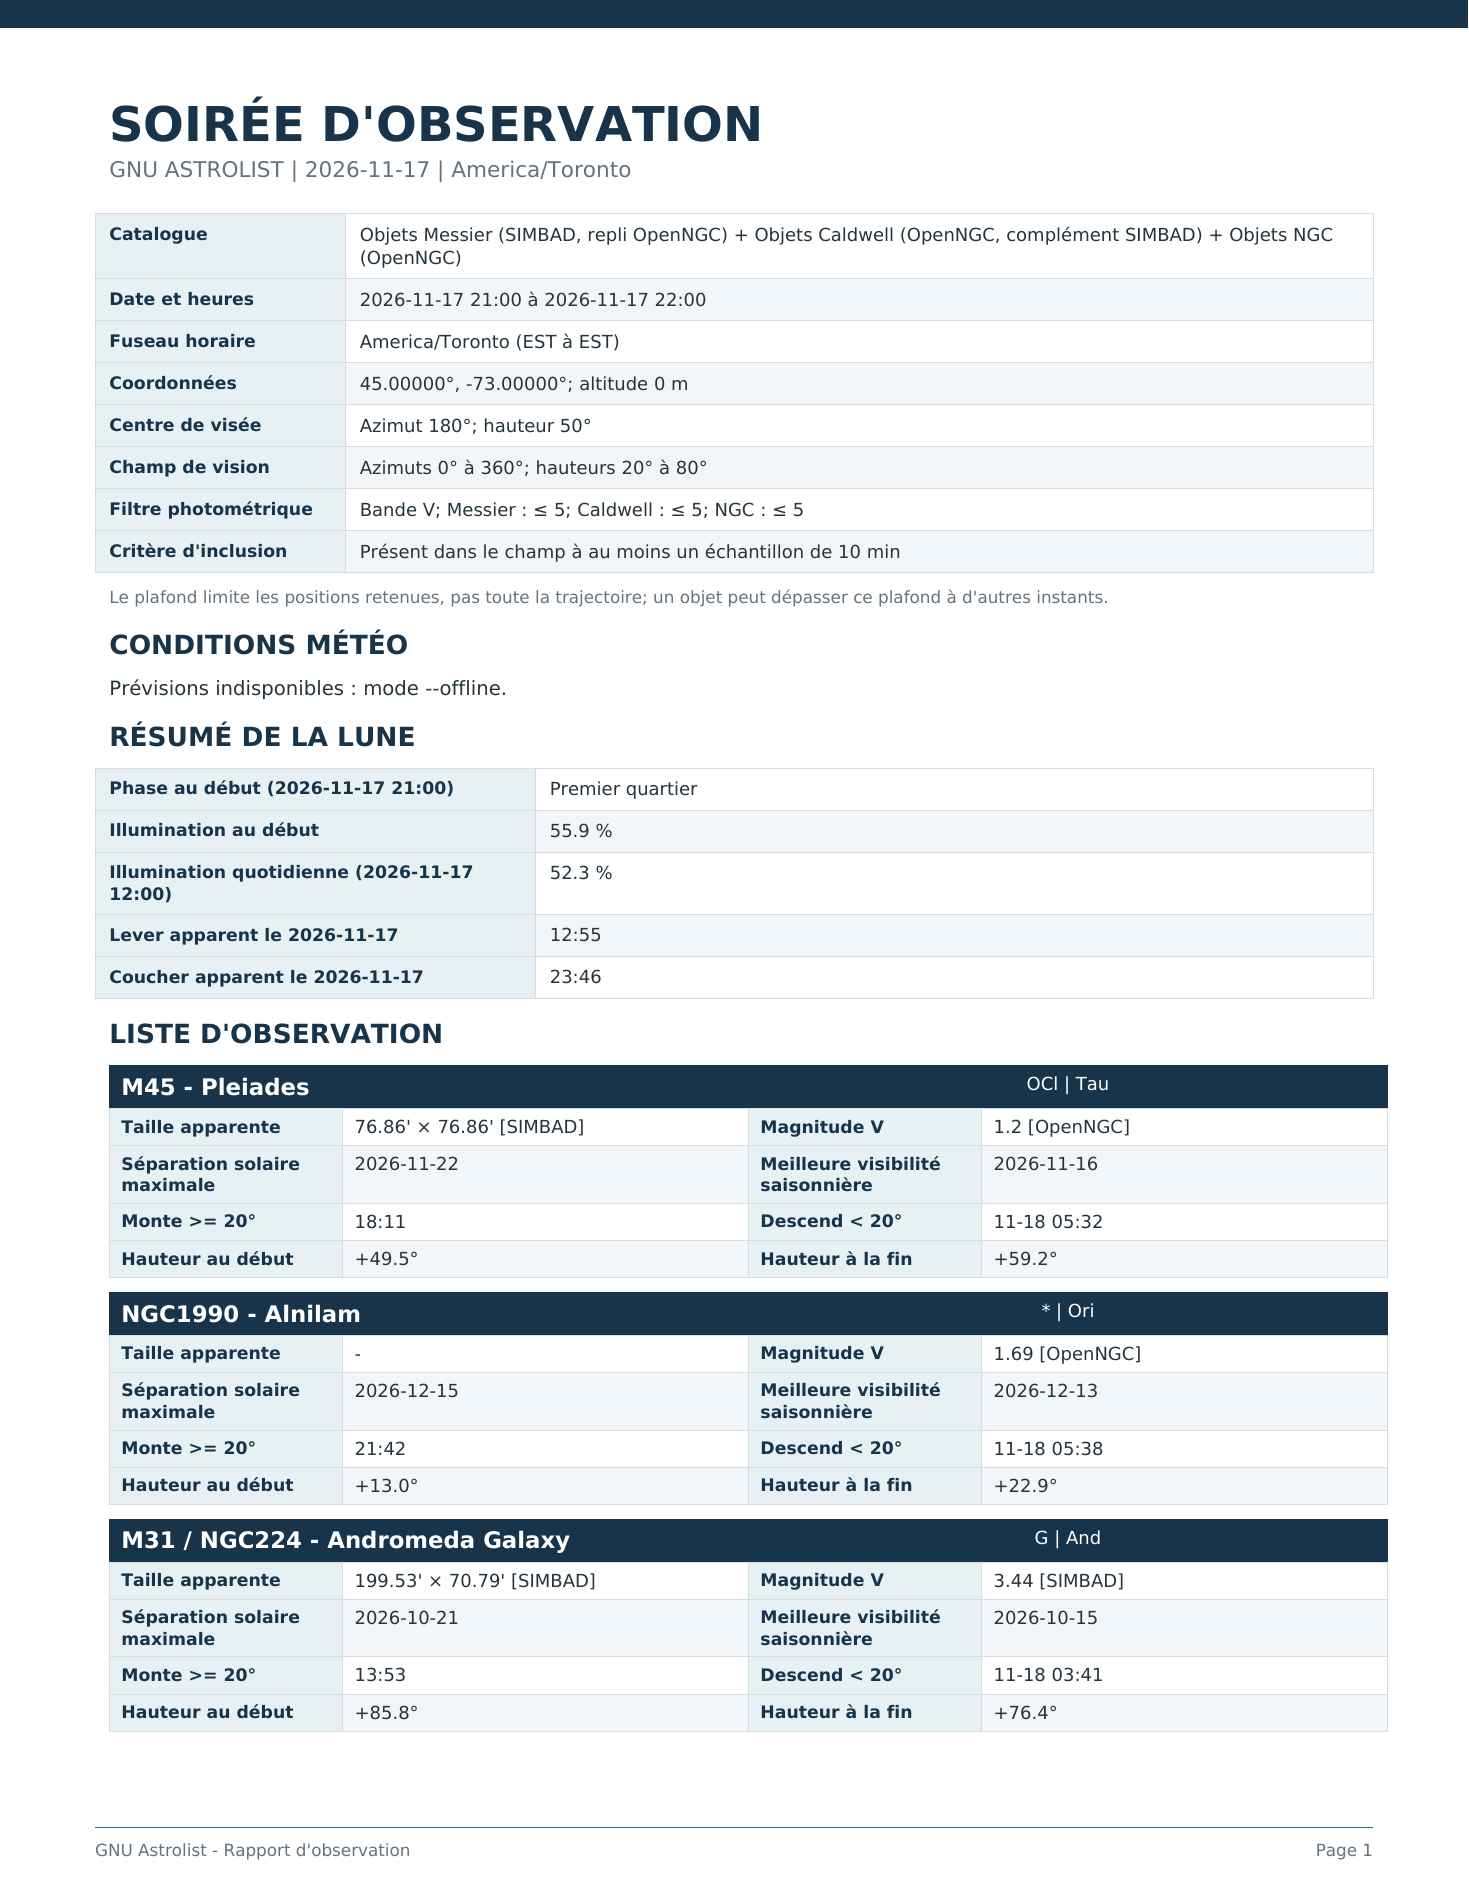
\includegraphics[width=.49\linewidth,height=24mm,keepaspectratio]{figures/image35.png}%
\end{column}\end{columns}
\end{frame}
\begin{frame}{Réutiliser ses poses brutes}
\vspace{-0.6mm}{\scriptsize\color{SwissMuted}1:53:30 – 1:57 · 3,5 min}\par\smallskip
\begin{columns}[T,onlytextwidth]\begin{column}{.38\textwidth}\raggedright\fontsize{9.6}{12}\selectfont
{\color{SwissAccent}\rule{6mm}{1pt}}\par\medskip
Retrouvez les prises du même champ sur plusieurs nuits.\par\medskip
Vérifiez date, filtre et durée avant de regrouper les images. Conservez les originaux.\par\medskip
\end{column}\begin{column}{.60\textwidth}\centering
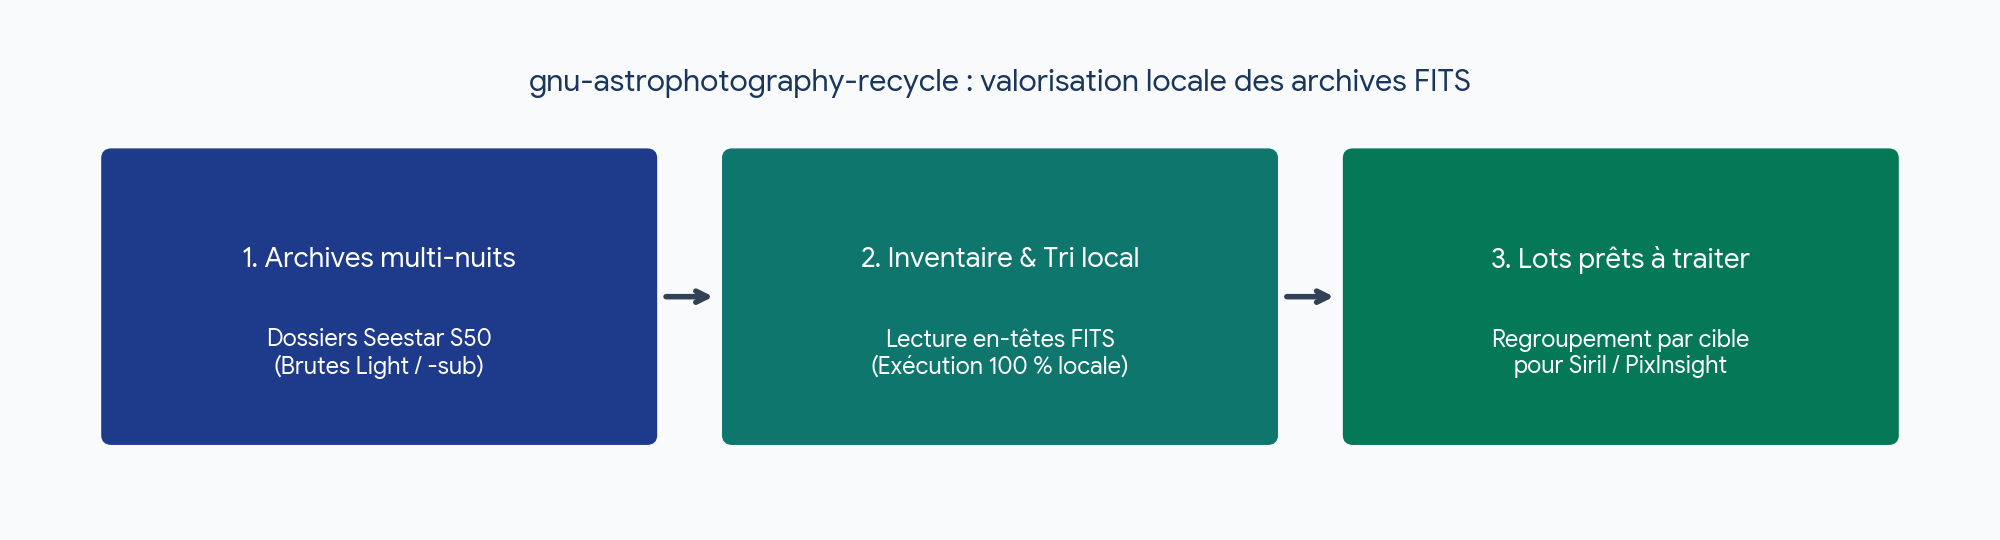
\includegraphics[width=1\linewidth,height=48mm,keepaspectratio]{figures/image36.png}%
\end{column}\end{columns}
\end{frame}
\begin{frame}{Que voulez-vous essayer à la prochaine Lune?}
\vspace{-0.6mm}{\scriptsize\color{SwissMuted}1:57 – 1:58:30 · 1,5 min}\par\smallskip
\begin{columns}[T,onlytextwidth]\begin{column}{.38\textwidth}\raggedright\fontsize{9.6}{12}\selectfont
{\color{SwissAccent}\rule{6mm}{1pt}}\par\medskip
Choisissez une tâche qui revient à chaque séance.\par\medskip
Formulez le résultat attendu en une phrase. Nommez une observation qui permettra de le vérifier.\par\medskip
\end{column}\begin{column}{.60\textwidth}\centering
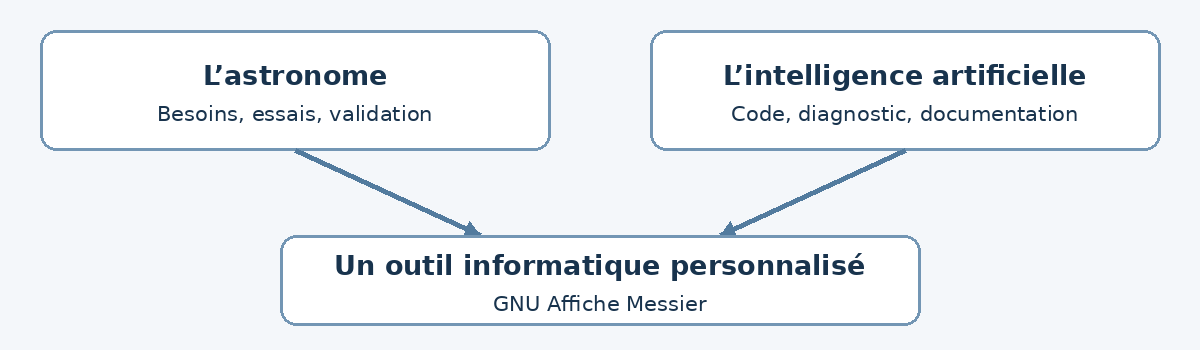
\includegraphics[width=1\linewidth,height=48mm,keepaspectratio]{figures/image1.png}%
\end{column}\end{columns}
\end{frame}
\begin{frame}{Retrouver les projets et les références}
\vspace{-0.6mm}{\scriptsize\color{SwissMuted}1:58:30 – 2:00 · 1,5 min}\par\smallskip
\begin{columns}[T,onlytextwidth]\begin{column}{.38\textwidth}\raggedright\fontsize{9.6}{12}\selectfont
{\color{SwissAccent}\rule{6mm}{1pt}}\par\medskip
Kim et Yegge (2025) : le modèle FAAFO.\par\medskip
Osmani (2025) : guider et vérifier le travail de l'IA.\par\medskip
Les 22 références figurent dans les notes. Scannez un code pour explorer les projets.\par\medskip
\end{column}\begin{column}{.60\textwidth}\centering

\includegraphics[width=1\linewidth,height=48mm,keepaspectratio]{figures/image37.png}%
\end{column}\end{columns}
\par\href{https://github.com/steveprudhomme}{\scriptsize github.com/steveprudhomme}
\end{frame}
\end{document}
